\documentclass[a4paper]{report} 
\usepackage[utf8]{inputenc}          
\usepackage[T1]{fontenc}
\usepackage[francais]{babel}
\usepackage[top=2cm, bottom=2cm, left=2cm, right=2cm]{geometry}
\usepackage{graphicx}
\usepackage{float}
\usepackage{amsmath}
\usepackage{wrapfig}
\usepackage{ccaption}
\usepackage[table]{xcolor} 
\usepackage{listings}
\usepackage[]{algorithm2e}
\usepackage{glossaries}

\newcommand{\HRule}{\rule{\linewidth}{0.5mm}}
\renewcommand{\thechapter}{\Roman{chapter}}
\addto\captionsfrench{\renewcommand{\chaptername}{Partie}}
\title{Rapport de stage}
\author{Zoé BRUNET}
\date{04/04/16 - 26/08/16}
\colorlet{punct}{red!60!black}
\definecolor{background}{HTML}{EEEEEE}
\definecolor{delim}{RGB}{20,105,176}
\colorlet{numb}{magenta!60!black}
\lstdefinelanguage{json}{
    basicstyle=\normalfont\ttfamily,
    numbers=left,
    numberstyle=\scriptsize,
    stepnumber=1,
    numbersep=8pt,
    showstringspaces=false,
    breaklines=true,
    frame=lines,
    backgroundcolor=\color{background},
    literate=
     *{0}{{{\color{numb}0}}}{1}
      {1}{{{\color{numb}1}}}{1}
      {2}{{{\color{numb}2}}}{1}
      {3}{{{\color{numb}3}}}{1}
      {4}{{{\color{numb}4}}}{1}
      {5}{{{\color{numb}5}}}{1}
      {6}{{{\color{numb}6}}}{1}
      {7}{{{\color{numb}7}}}{1}
      {8}{{{\color{numb}8}}}{1}
      {9}{{{\color{numb}9}}}{1}
      {:}{{{\color{punct}{:}}}}{1}
      {,}{{{\color{punct}{,}}}}{1}
      {\{}{{{\color{delim}{\{}}}}{1}
      {\}}{{{\color{delim}{\}}}}}{1}
      {[}{{{\color{delim}{[}}}}{1}
      {]}{{{\color{delim}{]}}}}{1},
}

\begin{document}

\begin{titlepage}
	\begin{figure}
		\hbox{
			\hspace*{1cm}
			
\includegraphics[width=3cm]{image/logo_centrale_nantes}
			\hspace{7cm}
			
\includegraphics[width=5cm]{image/logo_kisio} \\[2.5cm]
		}
	\end{figure}
	\begin{center}
	\textsc{\Large Rapport de stage ingénieur}\\[1cm]
	\textsc{\large 4 Avril 2016 — 26 Août 2016}\\[2cm]
 	\HRule \\[0.4cm]
		{\huge \bfseries Création d'une API isochrone}
	\HRule \\[2cm]	
	 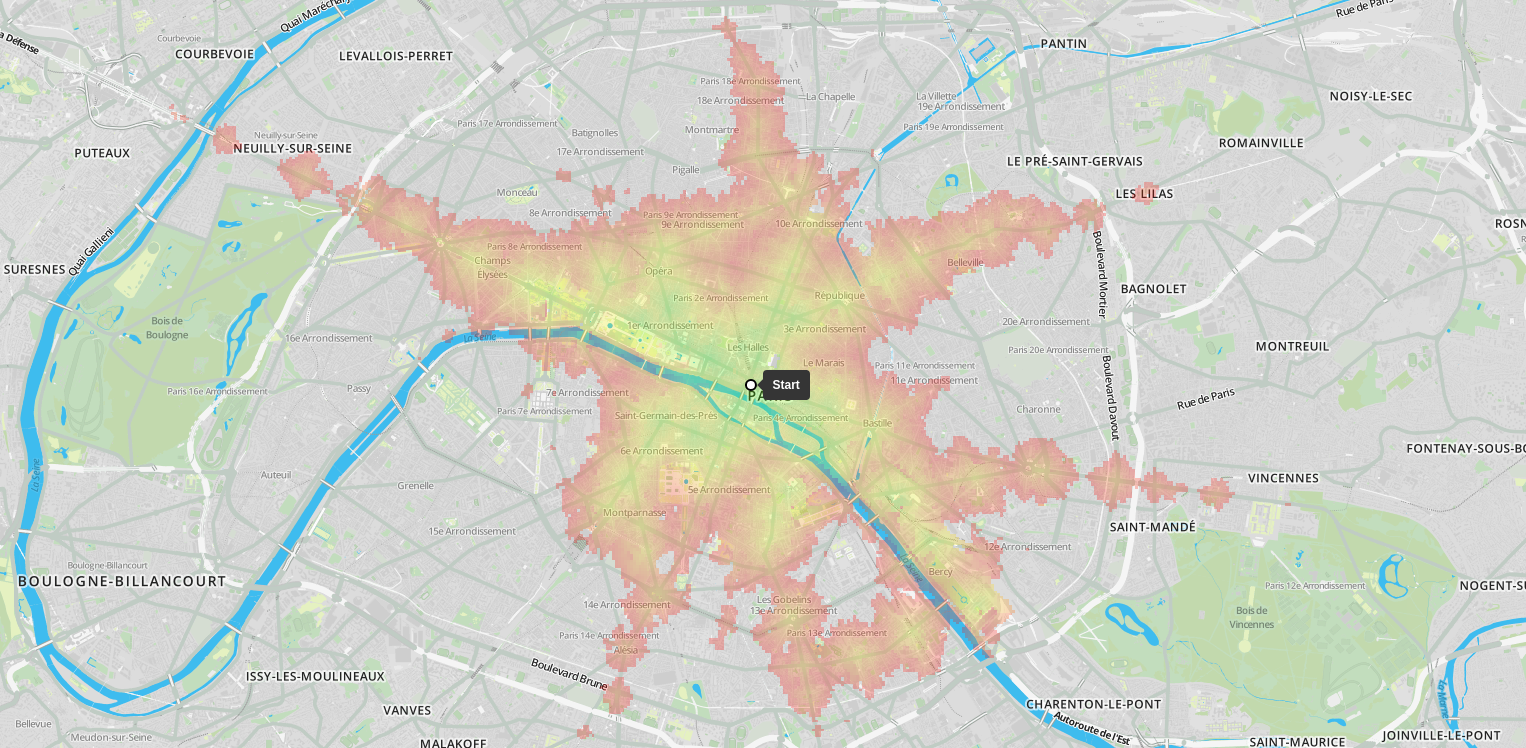
\includegraphics[width=\linewidth]{image/iso_garde}
    \\[1.6cm]
	    \begin{minipage}{0.46\textwidth}
      \begin{flushleft} \large
        Zoé \textsc{Brunet}\\
        \emph{Option :} urbaniSTIC\\
      \end{flushleft}
    \end{minipage}
    \begin{minipage}{0.46\textwidth}
      \begin{flushright} \large
        \emph{Tuteur entreprise :} Guillaume \textsc{Pinot}\\
        \emph{tutrice école : } Myriam \textsc{Servières}
      \end{flushright}
    \end{minipage}
        \vfill
    	\end{center}
\end{titlepage} 
\tableofcontents 
\newpage
\chapter*{Remerciements}
\addcontentsline{toc}{chapter}{Remerciements}

\paragraph{} Je tiens à remercier mon maître de stage Guillaume Pinot pour sa disponibilité, son sens de la pédagogie et ses démonstrations de yoyo en pause et en grooming.  Je souhaite remercier également Stephan Simart ou "chef" pour les intimes, ses remarques abondantes en démo et son point de vue marketing ont été bénéfiques pour ce stage.

\paragraph{} Je remercie tout particulièrement toute l'équipe de RO pour son accueil bienveillant. Grâce à leur curiosité et à leurs conseils je ne me suis jamais sentie trop bloquée. J'ai aimé la bonne ambiance au sein de l'équipe qui m'a permis de me sentir à l'aise tout au long de mon stage. Merci spécialement à Antoine et Pierre-Etienne pour m'avoir laissé gagner chaque fois que nous faisions la course à la piscine. Merci également à XL pour ses quizz C++, ses cours sur Pokemon Go et pour ne pas m'avoir laissée toute seule dans les bureaux en août.

\paragraph{} Merci à Nicolas Sirletti pour ses rappels sur le cours de traitement d'images et à Antoine Frediani pour son expertise Qgis.

\paragraph{} Enfin je remercie l'ensemble des professeurs de l'option urbaniSTIC pour cette année d'enseignement. J'ai découvert des problématiques inter disciplinaires qui m'ont réellement interessée et qui ont remis en question la vision que j'avais de la ville.	

\newpage

\chapter*{Introduction}
\addcontentsline{toc}{chapter}{Introduction}
	
\paragraph{} L'option urbaniSTIC a pour but d'enseigner à ses élèves comment utiliser de façon optimale les outils informatiques utiles dans les villes contemporaines. Au cours des sept mois passés au sein de cette formation j'ai pu m'interesser à diverses thématiques : politiques et problématiques urbaines, modélisation et représentation de la ville, acquisition et gestion de données. Lors de nombreux cours il a été souligné l'importance des transports en commun intra et inter urbain pour assurer la cohésion d'une ville. C'est pourquoi j'ai jugé interessant d'effectuer un stage dans une entreprise s'interessant aux systèmes d'infomations voyageurs (SIV).

\paragraph{} \emph{Kisio Digital} est un éditeur SaaS de solutions d’informations voyageurs multimodales. En plus de son domaine d'activité, c'est l'implication de cette entreprise dans l'open source, l'open service et l'open data qui m'a donné envie d'y faire mon stage. J'ai donc rejoint l'équipe de recherche opérationnelle en avril 2016 pour une durée de vingt-et-une semaines.

\paragraph{} Ce stage m'a permis d'approfondir les cours de programmation enseignés à l'Ecole Centrale de Nantes. J'ai pu y utiliser plusieurs langages comme Python, C++ et javascript. Je me suis également familiarisée avec la méthode agile utilisée dans de nombreuses entreprises d'informatique. 

\paragraph{} Ce rapport s’attachera à présenter le contexte de mon stage ingénieur, chez Kisio Digital. Il décrira la mise en place de deux nouvelles API calculant des isochrones dans le logiciel Navitia. Il expliquera le cheminement qui a été suivi afin de créer ces API et de les mettre en production.

\chapter{Contexte du stage}

\section{Présentation de Kisio Digital}
\subsection{Présentation générale}
			
\paragraph{} Pour mieux accompagner les autorités organisatrices de transports publics et de mobilité, le Groupe Keolis (leader  international du transport public de voyageurs) a regroupé ses expertises de Solutions et Services sous une marque unique, Kisio : Analysis, Consulting, Services, Solutions, et Digital. Kisio (650 collaborateurs et 60 millions de chiffre d'affaire) propose un ensemble de solutions et services aux acteurs de la mobilité.

\begin{figure}[H] 
	\begin{center}
		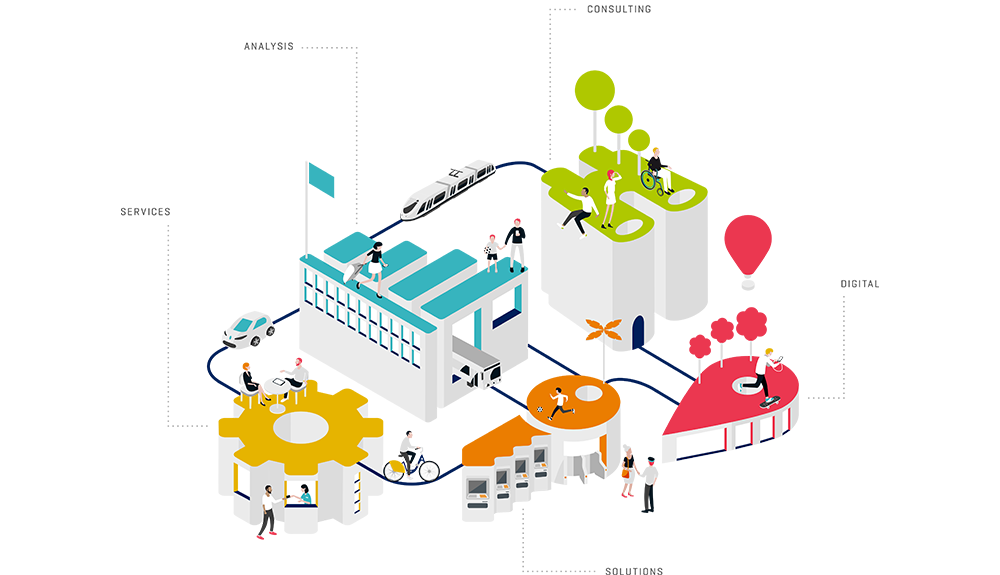
\includegraphics[width=500pt]{image/orga_kisio}
		\caption{Organisation au sein de Kisio}
		\label{Organisation au sein de Kisio}
	\end{center}
\end{figure}

\paragraph{} Mon stage a eu lieu chez Kisio Digital, leader de l'information voyageurs en France, et qui est une entreprise de services numériques. Elle édite des solutions de mobilité intelligente au service des voyageurs et des acteurs du transport depuis 15 ans. Plus concrètement, elle réalise  des sites web, des applis mobiles et des systèmes d’information voyageurs intégrant la recherche d’itinéraire multimodale et le temps réel, l’achat de titres de transport et bientôt le mobile-ticketing. Son domaine d’activité s’étend des réseaux de transports urbains et régionaux, aux réseaux ferroviaires nationaux (SNCF), en passant par les systèmes d’information voyageur des régions. 
				
\paragraph{} Kisio Digital encourage aussi l'innovation ouverte auprès des communautés de réutilisateurs de ses logiciels open source tels que Navitia et de son API navitia.io qui calcule 7 milliards d'itinéraires tous les ans.

\paragraph{} Par ailleurs Kisio Digital se définit comme le pionnier de la \emph{Responsive Locomotion} dont l'entreprise propose 4 définitions différentes et complémentaires\cite{ref_canal_tp} :

\begin{enumerate}
	\item La \emph{responsive locomotion} consiste à repenser les réseaux de transports à partir du contexte, des besoins et du point de vue de chaque voyageur.
	\item La \emph{responsive locomotion} est un ensemble d'outils qui visent à insuffler de l'agilité et de la souplesse dans les déplacements de chacun en autorisant les détours impromptus, en dessinant des parcours personnalisés, en organisant des déviations de dernière minute, etc.
	\item La \emph{responsive locomotion} est un projet qui englobe tous les moyens de transport : elle part du principe que le parcours et les besoins de chaque voyageur importent plus que le type de véhicule emprunté.
	\item La \emph{responsive locomotion} est une révolution d'interfaces et de services, dont l'ambition est de refonder la relation des hommes aux véhicules qui les meuvent.
\end{enumerate}

\subsection{L'information voyageur}

\paragraph{} Face à l'augmentation du nombre et de la complexité des déplacements, les clients souhaitent disposer d'une information fiable sur l'ensemble des modes de transport qui sont mis à leur disposition. Cette information multimodale est difficile à mettre en œuvre en raison du nombre important d'acteurs intervenant dans l'organisation des transports et de l'information et donc de la multiplicité des sources d’informations. En outre, la mise à jour des informations et la prise en compte des perturbations constituent un enjeu important d'un point de vue opérationnel, car les voyageurs ont besoin d'informations fiables avant et pendant le voyage.  

\paragraph{} Kisio Digital propose un panel de solutions permettant d'installer un service d'information voyageur performant et adapté à tous. Dans cette partie nous définierons brièvement les fonctions d'un tel système. 

\paragraph{} Un système d'information voyageur répond à trois besoins importants : 
				
\begin{description}
	\item[Simplifier la vie du voyageur:] Le voyageur peut préparer son itinéraire en toute sérénité. Il dispose de plusieurs informations lui permettant d'estimer la durée de son voyage mais également son coût, son impact sur l'environnement et les différents modes de transport qu'il va pouvoir emprunter.
	\item[Diminuer le stress :] L'opérateur de transport peut communiquer avec le voyageur pour le rassurer, le prévenir en cas de perturbation et lui proposer des itinéraires alternatifs.
	\item[Connaître les besoins de déplacement :] Les autorités organisatrices peuvent mieux adapter leur offre et répondre de façon optimale à la demande grâce aux informations remontées par les SIV.
\end{description}

\paragraph{} Historiquement les acteurs de la mobilité étaient issus soit du monde du transport public, soit de celui du vehicule particulier. L'information voyageur était une notion de transports publics et se présentait sous forme de fiches papier. Elle ne prenait pas en compte le temps réel et ne proposait aucune personnalisation. Avec la multimodalité due aux nouvelles mobilités, l'installation des Systèmes d'Aides à l'Exploitations et Informations Voyageurs (SAEIV) dans les années 2000  et à l'apparition du numérique la demande d'information voyageur a changé. Les SIV doivent maintenant être interactifs et proposer plusieurs services :
				
\begin{description}
	\item[Calculer des itinéraires:]  Il faut pouvoir poposer un "bon" itinéraire, mais cette notion est compliquée à définir. Il y a un compromis à faire entre l'itinéraire arrivant au plus tôt à destination, celui avec le moins de correspondances, le plus confortable, etc.
	\item[Accompagner le voyageur au cours du trajet :] Il faut pouvoir proposer en temps réel des alternatives en cas de perturbation sur l'itinéraire initialement prévu.
	\item[Informer sur l'accessibilité d'un lieu :] Le voyageur a besoin de connaître l'offre de transport à proximité de son point de départ.
\end{description}

\paragraph{} Les solutions proposées par Kisio Digital sont des solutions informatiques alimentées par le logiciel Navitia que nous décrirons plus en détail dans la partie suivante. 

\begin{figure}[H] 
	\begin{center}
		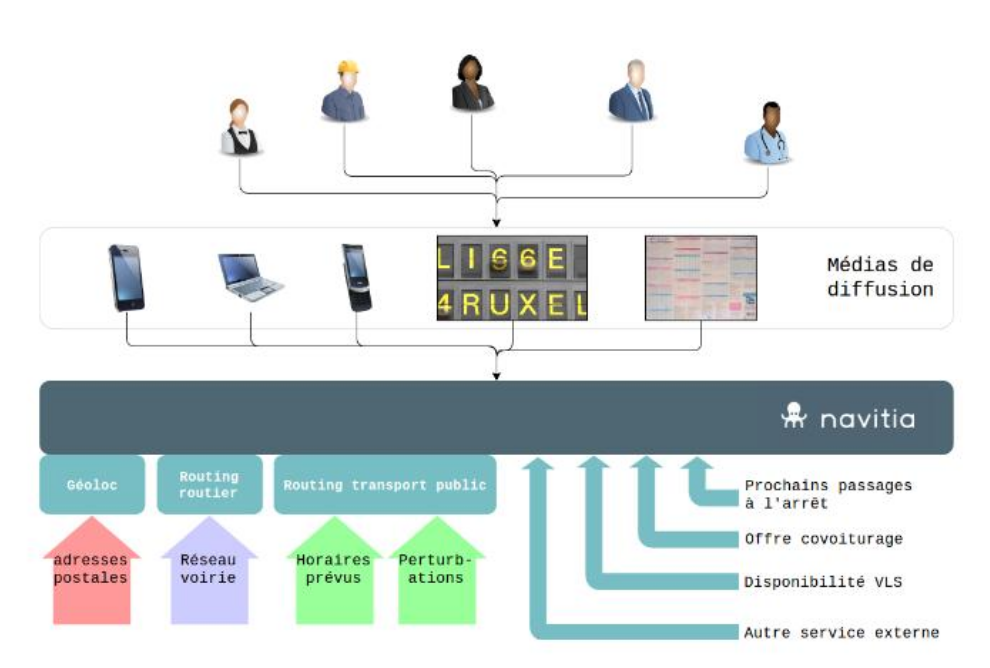
\includegraphics[width=300pt]{image/archi_SIV}
		\caption{Architecture du SIV proposé par Kisio Digital}
		\label{Architecture du SIV proposé par Kisio Digital}
	\end{center}
\end{figure}
\subsection{Organisation de l'équipe}

\paragraph{} L'organisation de l'équipe est ici présentée de façon sommaire et succinte. Bien qu'elle ne soit pas l'objet de mon stage, j'ai jugé intéressante de la décrire, d'autant qu'elle a fait l'objet d'une évolution au cours des cinq mois que j'ai passé à Kisio Digital.

\paragraph {}Depuis 2014, Kisio Digital a opéré des changements au sein de son entreprise pour adopter un mode de développement plus "agile":

\begin{quote}
"La méthode Agile est une méthode de gestion de projets Web introduite “officiellement” en 2001 avec la parution du “Manifesto for Agile Software Development” co-écrit par 17 grands acteurs du domaine de l’informatique et du développement de logiciel. Leur volonté était de proposer un nouveau mode de conception des programmes informatiques.

Cette méthode fonctionne sur la base de l'itératif et de l’incrémental, les tâches vont s’effectuer petit à petit, par ordre de priorité, avec des  phases de contrôle et d’échange avec le client."\cite{ref_agile}
\end{quote}

\paragraph{} La métode agile permet un dialogue plus riche entre le client et l'entreprise. A tout moment le client peut donner son opinion car il a régulièrement accès aux différentes versions fonctionnelles du logiciel. Les logiciels produits sont adaptés en fonction des retours clients et répondent donc précisément aux besoins exprimés. Elle repose en outre sur l'auto-organisation et donne plus de liberté aux développeurs et de visibilité sur le projet aux managers.


\paragraph {Organisation au sein d'une équipe} Le temps de travail chez Kisio Digital est donc rythmé par des \emph{sprints} d'une durée de 15 jours. Au début de chaque sprint les équipes se réunissent pour faire un \emph{sprint planning} où elles estimeront la durée et la difficulté des tâches qu'elles ont à réaliser. Ses tâches sont priorisées dans un \emph{backlog} en fonction des \emph{parties prenantes} où chaque équipe est représentée et remonte des besoins au moyen d'\emph{user stories}. Au sein de chaque équipe on trouve un \emph{Product Owner} qui est garant de la vision fonctionnelle de l'équipe. Lors du sprint l'équipe se réunit quotidiennement pour faire des \emph{stand up}, c'est à dire des réunions où tous les membres de l'équipe se coordonnent et donnent des informations sur leur avancement. Les membre de l'équipe font également des \emph{grooming} où ils se réunissent pour réévaluer le temps nécessaire à chaque user story, affiner les besoins qui y sont liés et les découper en sous-tâches. A l'issue de chaque sprint il faut présenter les traveaux effectués dans une \emph{démo} où les clients sont conviés. Après chaque démo l'équipe doit faire une \emph{rétros} pour discuter des points positifs et négatifs du sprint. C'est lors de ces rétro que les équipes décident d'\emph{actions} à mettre en place afin de rendre le sprint suivant encore plus performant.

\begin{wrapfigure}[15]{r}{8cm}
		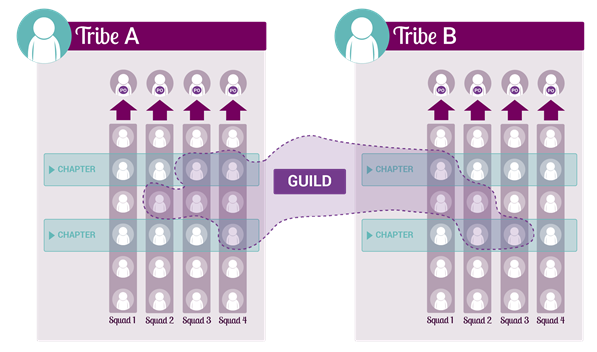
\includegraphics[width=8cm]{image/feature_team}
		\caption{Organisation des feature team}
		\label{Organisation des feature team}
\end{wrapfigure}

\paragraph {Feature team} Lorsque je suis arrivée chez Kisio Digital les équipes était organisées par produit dont elles étaient responsables et les membres de l'équipe avaient souvent des compétences similaires. J'étais par exemple dans l'équipe de Recherche Opérationnelle (RO) qui s'occupait du logiciel Navitia, tous les membres de cette équipe avaient des compétences en Python et en C++. En Juillet, Kisio Digital a changé son organisation pour faire des \emph{feature teams}. Les équipes ont été organisées autour de besoins, ce qui permettait, pour chaque user story, de modifier tous les produits impactés sans changer d'équipe. En outre ce type d'organisation permet une plus grande variété de profil au sein d'une même équipe. Cependant, pour garder la cohérence de chaque produit des \emph{guildes} se sont formées. Ainsi à partir de juillet 2016 les membres de l'ancienne équipe Navitia ont été répartis entre l'équipe itinéraire et l'équipe horaire mais ont aussi fondé la guilde Navitia pour pouvoir garder une interface cohérente au sein du logiciel.

\section{Navitia une API open source}

\paragraph{}La technologie Navitia est un agrégateur de données, qui facilite la création et l’exploitation de services d’information voyageur. Au-delà des fonctions de recherches d’itinéraires, cette solution offre toutes les fonctions permettant de prendre en compte les horaires adaptés (intégrant les différentes sources de perturbations), et l’ensemble des informations liées à l’accessibilité des transports, aux cheminements piétons ainsi que les tarifs. Navitia est d’ailleurs largement utilisé en France et couvre notamment les transports en commun de l’Ile de France.  

\begin{figure}[H] 
	\begin{center}
		
\includegraphics[width=100pt]{image/logo_navitia}
	\end{center}
\end{figure}

\subsection{Les API} 
\paragraph{} Navitia est un logiciel qui renvoit des flux faits pour être exploités par d'autres logiciels. On appelle cela une  \emph{API} (Application Programming Interface). L'API utilisant le logiciel Navitia s'appelle navitia.io. Ce sont ensuite les utilisateurs de navitia.io qui mettent en forme les flux retournés par l'API pour les présenter aux utilisateurs de leur application ou site web. 

\begin{figure}[H] 
	\begin{center}
		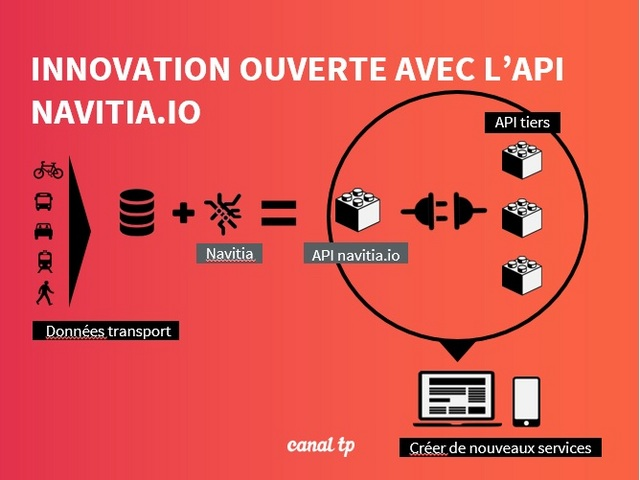
\includegraphics[width=300pt]{image/API_navitia}
		\caption{Innovation ouverte avec l'AI navitia.io}
		\label{Innovation ouverte avec l'AI navitia.io}
	\end{center}
\end{figure}

\paragraph{} En août 2016 navitia.io comptait 1400 réutilisateurs. Parmis eux on peut citer par exemple : destineo.fr, le site de calculateur d'itinéraires pour la région Pays de la Loire qui est utilisé par la TAN et Flat Turtle: une petite startup belge qui installe des écrans d’informations dans les halls d’entreprises. 

\subsection{L'open source, l'open data et l'open service}

\paragraph{} En 2012 Kisio Digital change de philosophie et se tourne vers l'open source. Un logiciel open source est un programme informatique dont le code source est distribué sous une licence permettant à quiconque de lire, modifier ou redistribuer ce logiciel. Le passage en open source a permis au logiciel de favoriser l’innovation du produit grâce à l’implication d’une communauté large de développeurs et d'assurer une pérennité de la solution pour tous ses clients. 

\paragraph{} En restant dans cet esprit, Kisio Digital est maintenant un fournisseur d'open data. L'open data consiste a rendre accessible à tous des données, ici géographiques, rassemblées par une organisation. Cependant Kisio Digital ne va pas sur le terrain pour collecter les données qu'il met en open data. Grâce à son logiciel Fusio, l'entreprise agrège différentes sources de données dans différents formats pour produire un fichier au format gtfs et un autre au format ntfs. Ces deux fichiers ainsi que toutes les données open data dont fusio s'est servi sont disponible gratuitement et librement sur le site navitia.io.

\paragraph{} Enfin navitia.io est un open service. le site met à disposition de tous les services fournis par le logiciel Navitia. L'utilisateur peut ensuite utiliser Navitia qui est alimenté par les données open data fournies par Kisio Digital. 

\subsection{Le logiciel Navitia}

\paragraph{} L'architecture du logiciel Navitia a beaucoup évolué ces dix dernières années.

\begin{figure}[H]
	\begin{center}
		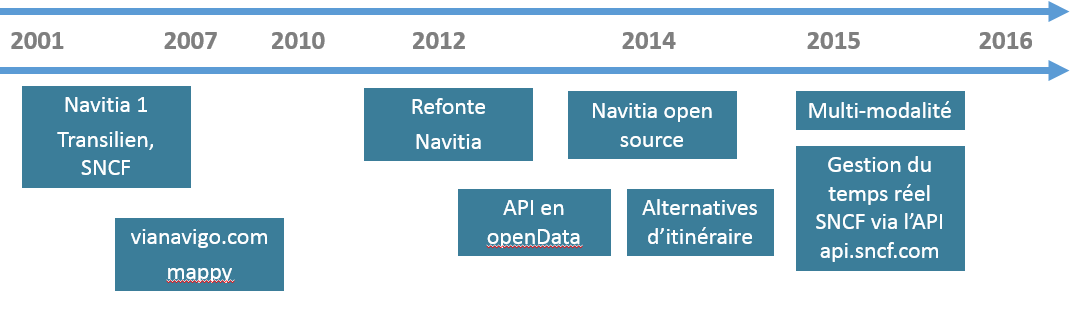
\includegraphics[width=400pt]{image/historique_navitia}
		\caption{Historique de Canal tp}
		\label{Historique de Canal tp}
	\end{center}
\end{figure}


\paragraph{}Navitia repose sur un calculateur codé en C++ nommé Kraken et une interface : Jörmungandr codée en python. Avant tout calcul, tartare un autre logiciel, crée une base de données à partir de fichier ntfs. Le format ntfs a été créé pour Navitia et est assez proche du format gtfs. Les données liées à la topologie des territoires et au filaire de voierie sont extraite d'open street map qui est une base de données gégraphiques collaborative, celles liées aux réseaux de transport sont fournies par les opératuers de transport (SAEIV, ...).

\begin{figure}[H]
	\begin{center}
		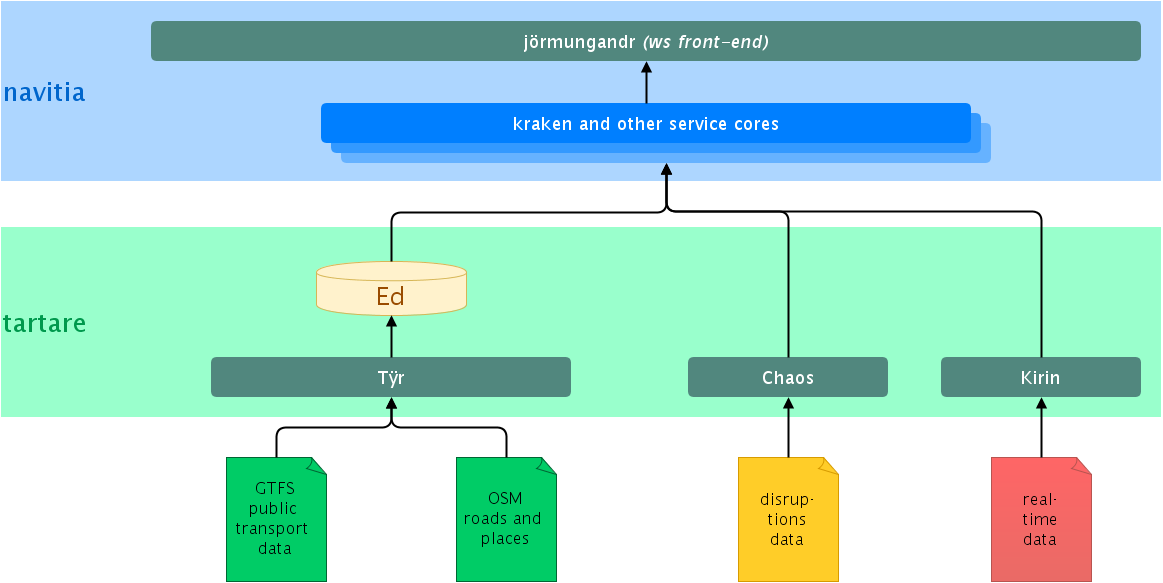
\includegraphics[width=400pt]{image/architecture_navitia}
		\caption{Architecture de Navitia}
		\label{Architecture de Navitia}
	\end{center}
\end{figure}

\paragraph{} Le calcul d'itinéraire qui est fait dans Kraken est basé sur l'algorithme RAPTOR. Kraken lit et interprète ensuite les itinéraires pour que Jörmungandr ne renvoie que les meilleurs itinéraires en fonction du profil du voyageur. Les informations sont échangées entre Jörmungandr et Kraken via des flux sérialisés au format protocol buffers.

\section{Présentation du stage}

L'intitulé de mon stage était le suivant :

\begin{quote}
	\emph{"Simplification dans l’utilisation du service Isochrone de l’API de web-service http://api.navitia.io. Le stage concerne la simplification de l’utilisation du service "isochrone" qui permet de remonter les temps d'accès depuis un point donné vers toute destination. Il consiste à transformer la sortie actuelle de Navitia (qui est un tableau de point avec pour chacun une heure d'arrivée) en éléments graphiques vectoriels permettant de dessiner une carte, plus simple à intégrer. Il nécessite de manipuler principalement du code c++, ainsi que du code Python, des librairies de cartographie et des bases de données."}
\end{quote}

\paragraph{} Ce stage implique de coder dans Kraken afin de récupérer les isochrones déjà calculés par l'algorithme RAPTOR pour les traiter et les organiser de manière à rendre ces informations plus visuelles. Il faut ensuite coder dans Jörmungandr afin d'implémenter la nouvelle API. 

\chapter{Déroulement du stage}

\section{Définition des nouvelles API}

\subsection{Les isochrones}

\paragraph{}Les isochrones sont des courbes permettant de mesurer l'accessibilité d'un lieu en terme de temps. Ils partent du principe que la proximité géographique de deux lieux n'implique pas nécessairement qu'il sera rapide d'aller de l'un à l'autre. Les isochrones permettent de raisonner en terme de temps d'accès plutôt qu'en terme de distance.

\paragraph{}La définition comunément admise en cartographie pour un isochrone est : ensemble des points atteignables en un temps donné en partant d'un point donné. Cette définition n'est pourtant pas satisfaisante si on l'applique aux transports en commun. 

\paragraph{}En effet contrairement au mode de transport tel que le vélo, la marche à pied ou la voiture, on ne peut pas se contenter de réfléchir en terme de durée lorsqu'on prend les transport en commun. Selon l'heure de départ ou d'arrivé souhaitée par le voyageur l'offre de transport ne sera pas la même. Par conséquent le temps de trajet dépend de l'horaire pendant lequel ce trajet est effectué. Dès lors il faut redéfinir notre notion d'isochrone : un isochrone est l'ensemble des points atteignables en un temps donné en partant d'un point donné à une date et un horaire donné.

\begin{figure}[H]
	\begin{minipage}[c]{.46\linewidth}
		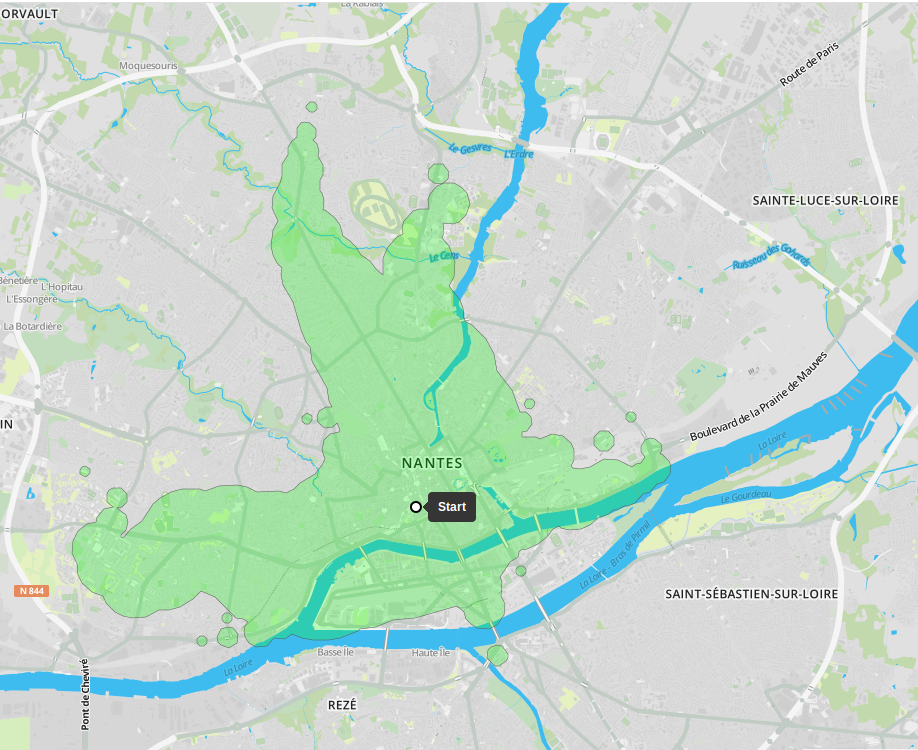
\includegraphics[width=8cm]{image/iso_8h}
       		\caption{Isochrone à 8h00}
		\label{Isochrone à 8h00}
	\end{minipage} \hfill
	\begin{minipage}[c]{.46\linewidth}
		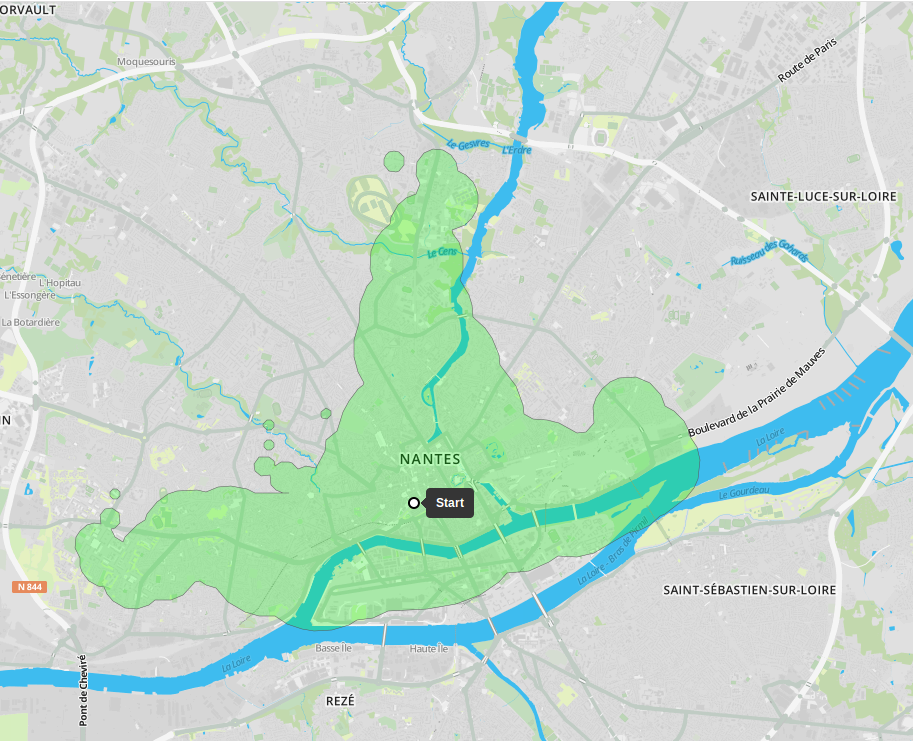
\includegraphics[width=8cm]{image/iso_00h30}
       		\caption{Isochrone à 00h30}
		\label{Isochrone à 00h30}
	\end{minipage}
	\legend{Isochrones de 10 minutes partant de Commerce}
\end{figure}

\paragraph{} Selon les usages qui en seront fait la définition des isochrones peut être étendue. Dans ce stage nous avons définit deux usages et donc deux types d'isochrones bien distincts : 

\paragraph{Les isochrones vectoriels} Du début de mon stage à juin 2016 j'ai considéré qu'un isochrone permettait de repérer des services à proximité d'un point de départ. Ces isochrones sont des multipoligones utilisés pour calculer des intersections avec d'autres données vectorielles. A chaque isochrone correspond une et une seule durée qui est la durée maximale souhaitée par l'utilisateur. On peut par exemple souhaiter savoir où se trouvent les boulangeries à moins de 10 minutes de son lieu de travail. Pour celà on trace un isochrone de 10 minutes autour de ce lieux et on sélectionne les boulangeries à l'interieur du multipolygone ainsi obtenu.

\paragraph{Les  heat maps} De juin à la fin de mon stage je me suis concentrée sur des isochrones permettant des tracés cartographiques plus précis. Cette fois il n'y a plus une seule durée. Le but est en un seul appel à l'API d'obtenir des données permettant de tracer une carte de chaleur selon le temps d'accés de chaque points. Contrairement à l'isochrone précédent la donnée en sortie de l'API n'est plus vectorielle.

\begin{figure}[H]
	\begin{minipage}[c]{.46\linewidth}
		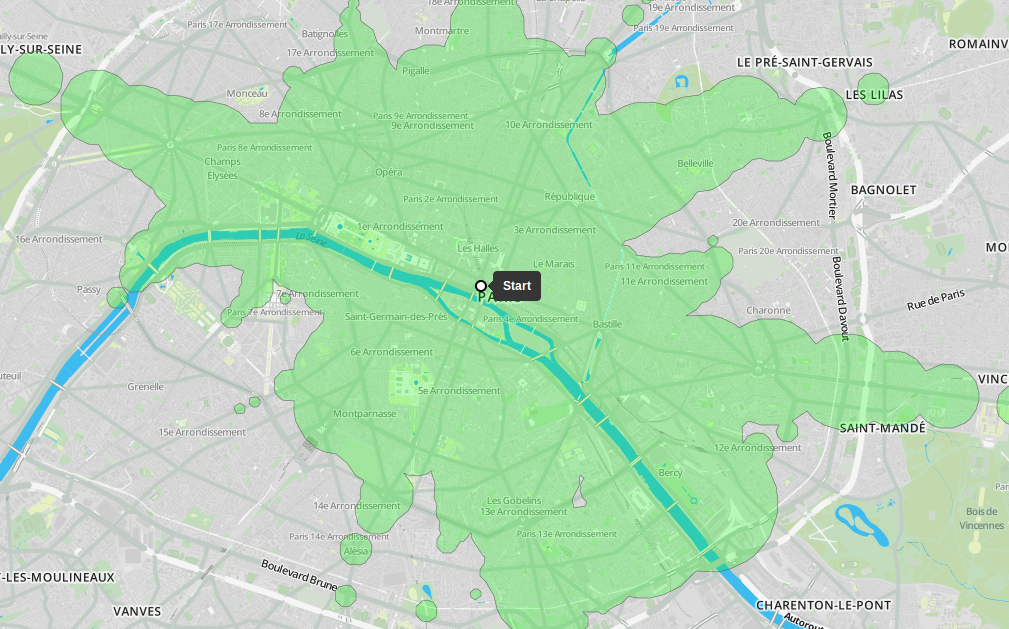
\includegraphics[width=8cm]{image/iso_vect}
       		\caption{Isochrone vectoriel}
		\label{Isochrone vectoriel}
	\end{minipage} \hfill
	\begin{minipage}[c]{.46\linewidth}
		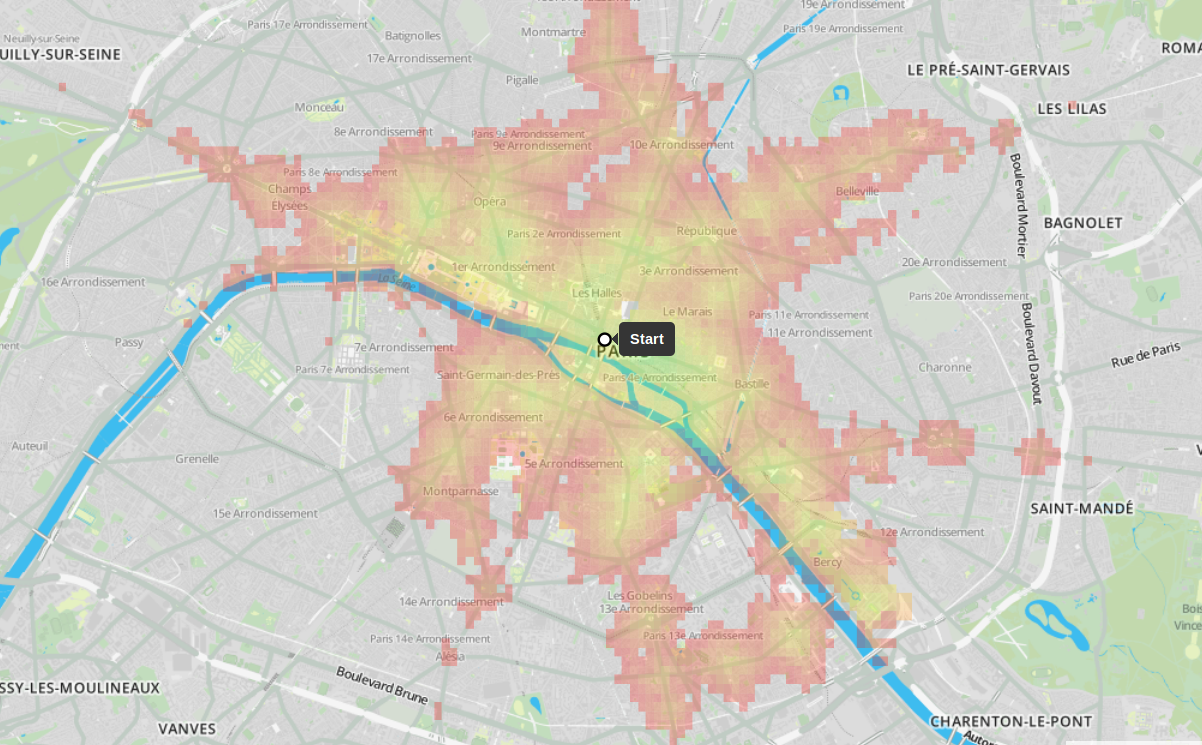
\includegraphics[width=8cm]{image/heat_map}
       		\caption{Heat map}
		\label{Heat map}
	\end{minipage}
	\legend{Isochrones de 20 minutes partant de Châtelet à 8h00}
\end{figure}

\subsection{Les problématiques d'interface}

\paragraph{} Comme nous l'avons vu dans la présentation de Navitia, l'architecture du logiciel est assez complexe. La première étape de mon stage consistait donc à spécifier les paramètres d'entrée et de sortie de l'API. Ces paramètres ont été afinés tout au long du stage et ceux présentés dans cette partie correspondent à ceux qui ont été retenus à la fin de mon stage et different légèrement de ceux définis au début de mon stage. 

\paragraph{} Navitia est un unique logiciel qui propose différents services: calcul d'itinéraires, autocomplétion, affichage des horaires d'une ligne de bus, ... Pour que le logiciel reste facilement utilisable il est nécessaire que toutes les APIs soient cohérentes entre elles. Cela signifie : que les APIs doivent être nommées selon la même sémantique, que le nom des paramètres ne doit pas changer d'une API à l'autre, que le cheminement pour accéder à une API doit toujours être le même. Il faut aussi que les noms propres à chaque API soient clairs et sans équivoques. 

\paragraph{Quelques règles à respecter} Pour le choix des noms des paramètres d'une API dans Navitia il y a quelques règles à respecter : les paramètres qui peuvent être appelés plusieurs fois sont suivis de crochets \emph{exemple: first\_section\_mode[]}. Les paramètres avancés et ne servant qu'aux développeurs (par exemple pour debuguer) sont précédés d'un underscore \emph{exemple: \_current\_datetime}. Le nom des APIs et de leurs paramètres sont en snake case et au pluriel\emph{exemple: heat\_maps}.

\paragraph{} Outres les paramètres indispensables à la construction d'un isochrone que nous avons vu dans la partie précédente, il a fallu adapter les paramètres utilisés dans le calcul d'itinéraire afin de maintenir la cohérence de l'interface. Voici un tableau des différents paramètres implémentés :

\definecolor{LightCyan}{rgb}{0.88,1,1}
\begin{center}
	\begin{tabular}{|l|l|p{1.5cm}|p{6cm}|l|}
	\hline
	\multicolumn{5}{|c|}{\cellcolor{LightCyan} \textbf{Paramètres communs aux API isochrones et heat\_maps}} \\
	\hline
	\textbf{Requis} & \textbf{Nom} & \textbf{Type} & \textbf{Description} &  \textbf{valeur par défault} \\
	\hline
	non & from & id & Identifiant du point de départ de l'isochrone. &\\
	\hline
	non & to & id & Identifiant du point d'arrivé de l'isochrone, ce paramètre est utilisé quand on calcule un isochrone inverse. &\\
	\hline
	oui & datetime & iso-date-time & Date et horaire d'arrivée ou de départ de l'isochrone. & \\
	\hline
	non & forbidden\_uris[] & id & Identifiant permetant d'éviter une ligne, un mode, un réseau, etc. & \\
	\hline
	non & first\_section\_mode[] & tableau de string & Force le premier mode de rabattement qui n'est pas du transport en commun.  ce paramètre peut prendre les valeurs suivantes : \emph{walking, car, bike, bss}. Bss correspond aux vélos en libre service. Cest un tableau, il peut donc y avoir plusieurs modes séléctionnés.
	\paragraph{}\emph{Note :} Choisir bss implique que la marche est également autorisée puisqu'il faut marcher pour aller jusqu'à la station des vélos en libre service.
	\paragraph{}\emph{Note 2 :} Le paramètre est inclusif et non exclusif, donc pour exclure un mode il faut ajouter tous les autres modes & walking \\ 
	\hline
	non & last\_section\_mode[] & tableau de string & Comme first\_section\_mode[] mais pour le rabattement en fin d'itinéraire. & walking \\ 
	\hline
	non & max\_transferts & int & Nombre de correspondances maximum autorisées. & \\
	\hline
	non & max\_duration\_to\_pt & int & Durée maximum de rabattement pour atteindre un transport public afin de limiter la marche à pied ou le vélo. Son unité est la seconde
	\paragraph{}\emph{Note :} On peut règler indépendemment la durée maximale de rabattement pour chaque mode en utilisant les paramètres : \emph{max\_walking\_duration\_to\_pt}, \emph{max\_bike\_duration\_to\_pt}, \emph{max\_bss\_duration\_to\_pt}, \emph{max\_car\_duration\_to\_pt} & 15*60s \\
	\hline
	non & walking\_speed & float & Vitesse de marche à pied en m/s & 1.12 m/s (4km/h) \\
	\hline
	non & bike\_speed & float & Vitesse en vélo en m/s & 4.1 m/s (14.7 km/h) \\
	\hline
	non & bss\_speed & float & Vitesse en vélo en libre service en m/s & 4.1 m/s (14.7 km/h) \\
	\hline
	non & car\_speed & float & Vitesse en voiture en m/s & 16.8 m/s (60 km/h) \\
	\hline
	non & data\_freshness & enum & Permet d'utiliser les données temps réel ou les données théoriques. data\_freshness peut prendre deux valeurs : \emph{realtime} ou \emph{base\_schedule} & base\_schedule \\
	\hline
	non & traveler\_type & enum & C'est un profil prédéfini où les paramètres \emph{first\_section\_mode[]}, \emph{last\_section\_mode[]}, \emph{walking\_speed}, \emph{bike\_speed} et \emph{bss\_speed} sont modifiés en fonction de la valeur choisie. Les valeurs possibles sont : \emph{standard}, \emph{slow\_walker}, \emph{fast\_walker} et \emph{luggage} & standard \\
	\hline
	\end{tabular}
\end{center}

\begin{center}
	\begin{tabular}{|l|l|p{1.5cm}|p{6cm}|l|}
	\hline
	\multicolumn{5}{|c|}{\cellcolor{LightCyan} \textbf{API isochrones}} \\
	\hline
	\textbf{Requis} & \textbf{Nom} & \textbf{Type} & \textbf{Description} &  \textbf{valeur par défault} \\
	\hline
	non & max\_duration & int & Durée maximale de l'isochrone en secondes &\\
	\hline
	non & min\_duration & int & Durée minimale de l'isochrone en secondes & 0 secondes\\
	\hline
	non & Boundary\_duration[] & int & Pour faire plusieurs isochrones en une requête (limité à 10 \emph{boundary\_duation[]} par requête) & \\
	\hline
	\end{tabular}
\end{center}

Aucun de ces paramètres n'est obligatoire individuellement mais on ne peut pas faire un isochrone sans un paramètre \emph{max\_duration} ou \emph{boundary\_duration[]}. De plus tous les \emph{boundary\_duration[]} ayant une valeur suppérieure au paramètre \emph{max\_duration} (s'il est renseigné) seront ignorés. 

\begin{center}
	\begin{tabular}{|l|l|p{1.5cm}|p{6cm}|l|}
	\hline
	\multicolumn{5}{|c|}{\cellcolor{LightCyan} \textbf{API heat\_maps}} \\
	\hline
	\textbf{Requis} & \textbf{Nom} & \textbf{Type} & \textbf{Description} &  \textbf{valeur par défault} \\
	\hline
	oui & max\_duration & int & Durée maximale de l'isochrone en secondes &\\
	\hline
	non & resolution & int & Nombre de pixels sur une ligne ou une colonne de la grille qui sert à tracer l'isochrone & 500\\
	\hline
	\end{tabular}
\end{center}

\subsection{La réponse de l'API}

\subsubsection{API isochrones} 

\paragraph{}Navitia renvoit un \emph{flux json} quel que soit l'API requétée. Il fallait donc trouver le moyen de renvoyer des informations géographiques dans un tel flux. Le format geojson convenait parfaitement à ces critère.

\begin{quote}
	\emph{GeoJSON (de l'anglais Geographic JSON, signifiant littéralement JSON géographique) est un format ouvert d'encodage d'ensemble de données géospatiales simples utilisant la norme JSON (JavaScript Object Notation).\cite{ref}.}
\end{quote}


\paragraph{} Pendant les trois premiers mois de mon stage j'ai mis en place une première API \emph{isochrones} qui traçait des cercles tout autour des points d'arrêt atteignables en transport en commun. En faisant varier le rayon de ces cercles en fonction du temps d'accès à ce point d'arrêt on obtient une assez bonne estimation des différents lieux accessibles en un temps donné.

\begin{figure}[H]
	\begin{center}
		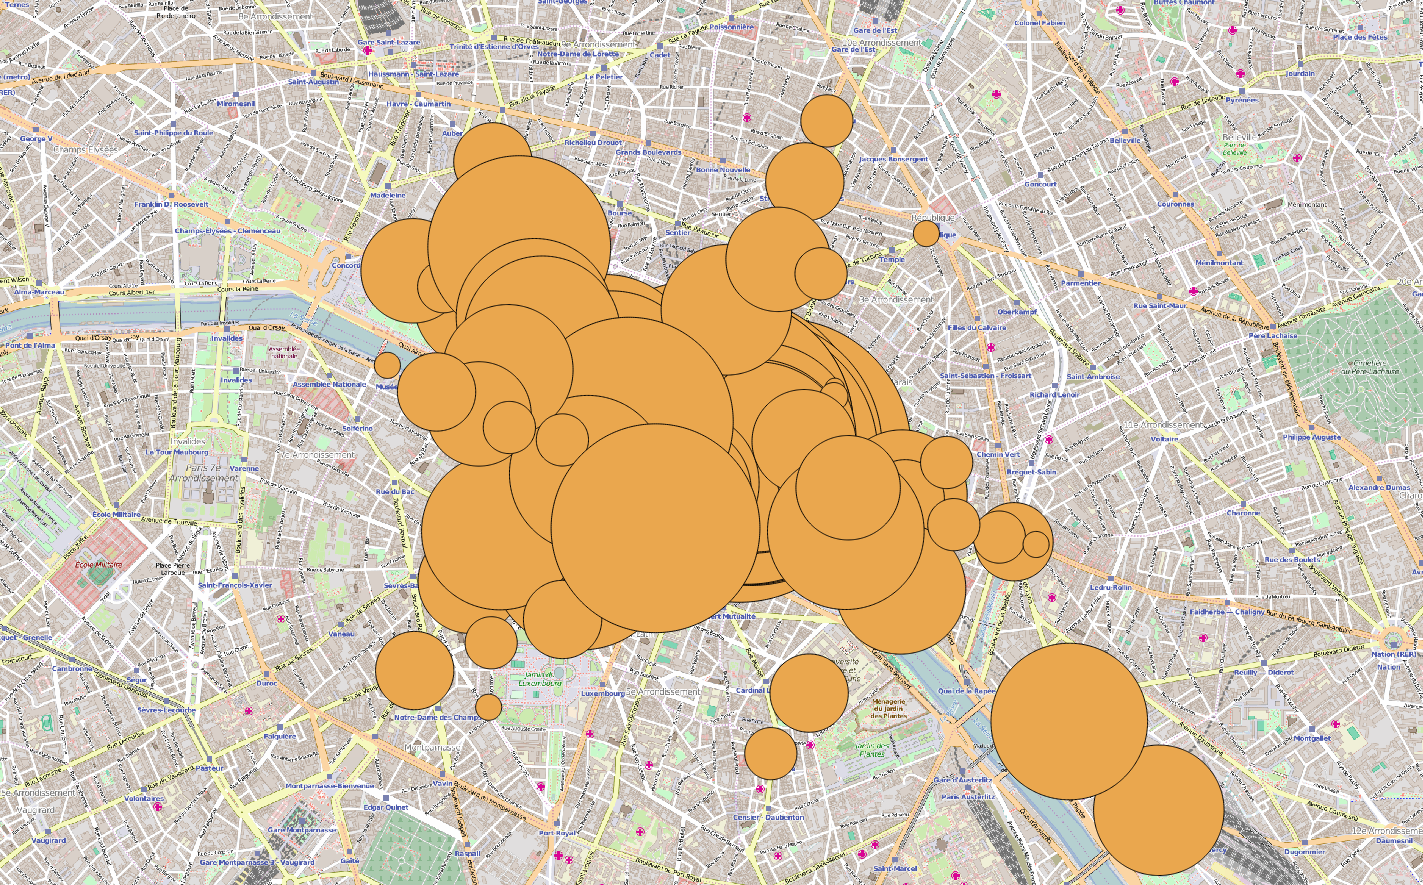
\includegraphics[width=400pt]{image/premiers_isochrones}
		\caption{Cercles autour des points d'arrêt}
		\label{Cercles autour des points d'arrêt}
	\end{center}
\end{figure}

\paragraph{} Pour avoir un rendu plus agréable et pour n'avoir qu'un seul objet à manier on fusionne ces cercles en un multi polygone.

\begin{figure}[H]
	\begin{center}
		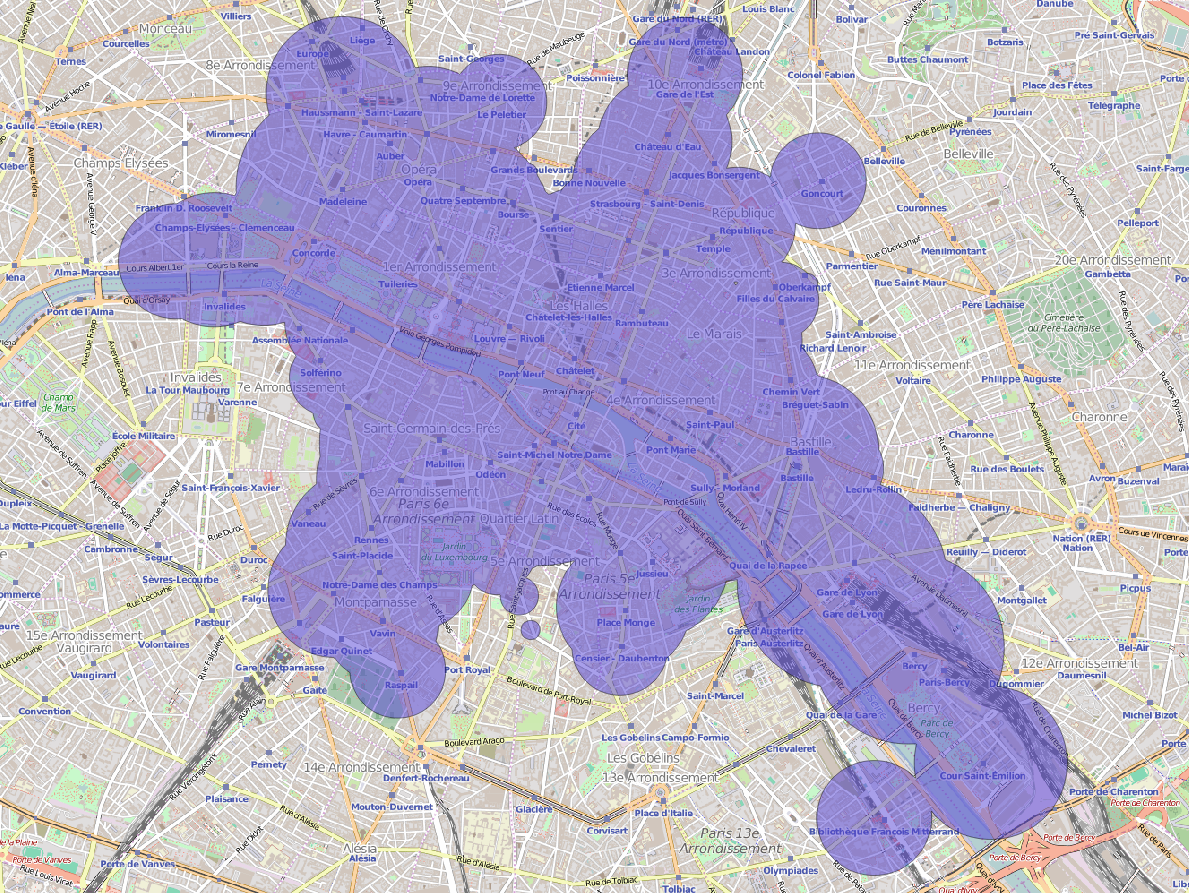
\includegraphics[width=300pt]{image/iso_merged}
		\caption{Multipolygone obtenu après fusion des cercles}
		\label{Multipolygone obtenu après fusion des cercles}
	\end{center}
\end{figure}

\paragraph{} Généralement, il est intéressant de tracer plusieurs isochrones à différentes durées maximales. Mais pour afficher ensemble et correctement plusieurs isochrones il ne faut pas qu'il y ait de chevauchement entre eux puisque leur transparence s'ajouteraient et rendraient la carte dificilement lisible.

\begin{figure}[H]
	\begin{center}
		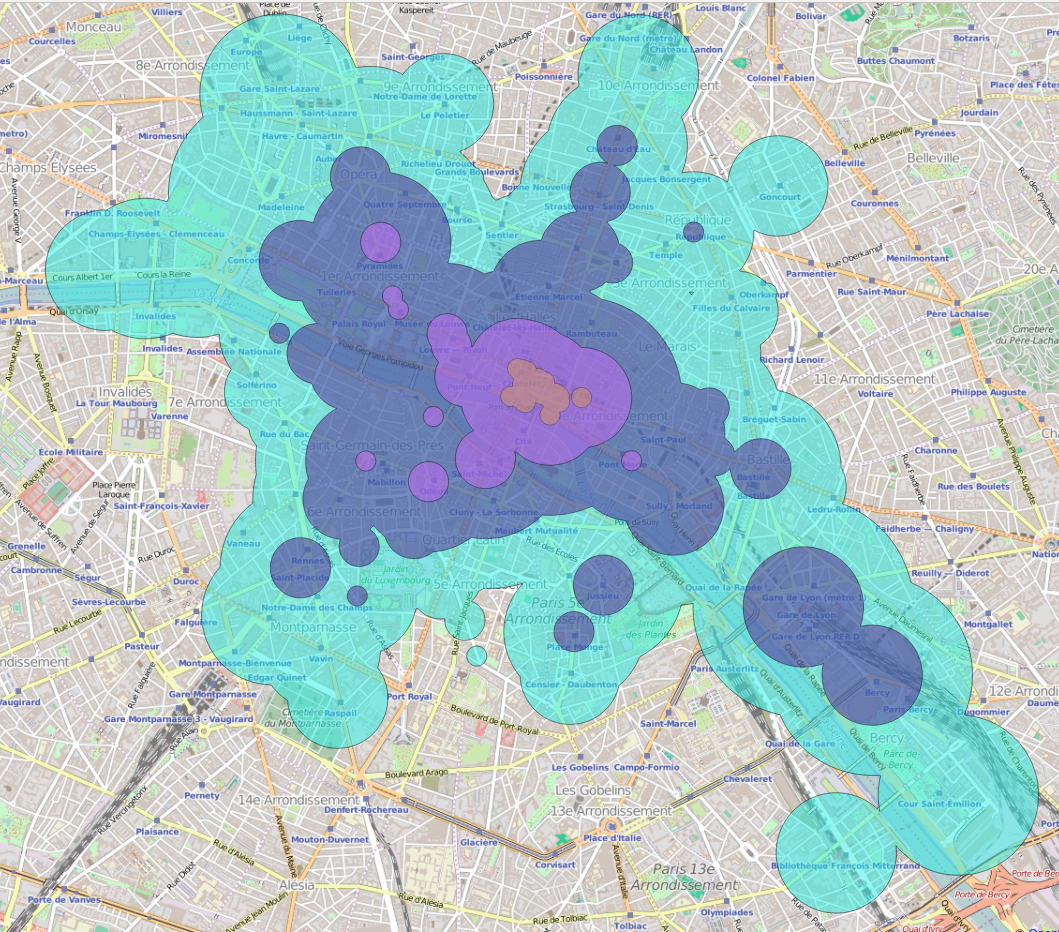
\includegraphics[width=300pt]{image/multi_iso}
		\caption{Multiisochrone}
		\label{Multiisocrone}
	\end{center}	
\end{figure}

\paragraph{} Pour résoudre ce problème une borne min a été implémenté, elle permet de tracer un isochrone entre deux durées. 

\begin{figure}[H]
	\begin{center}
		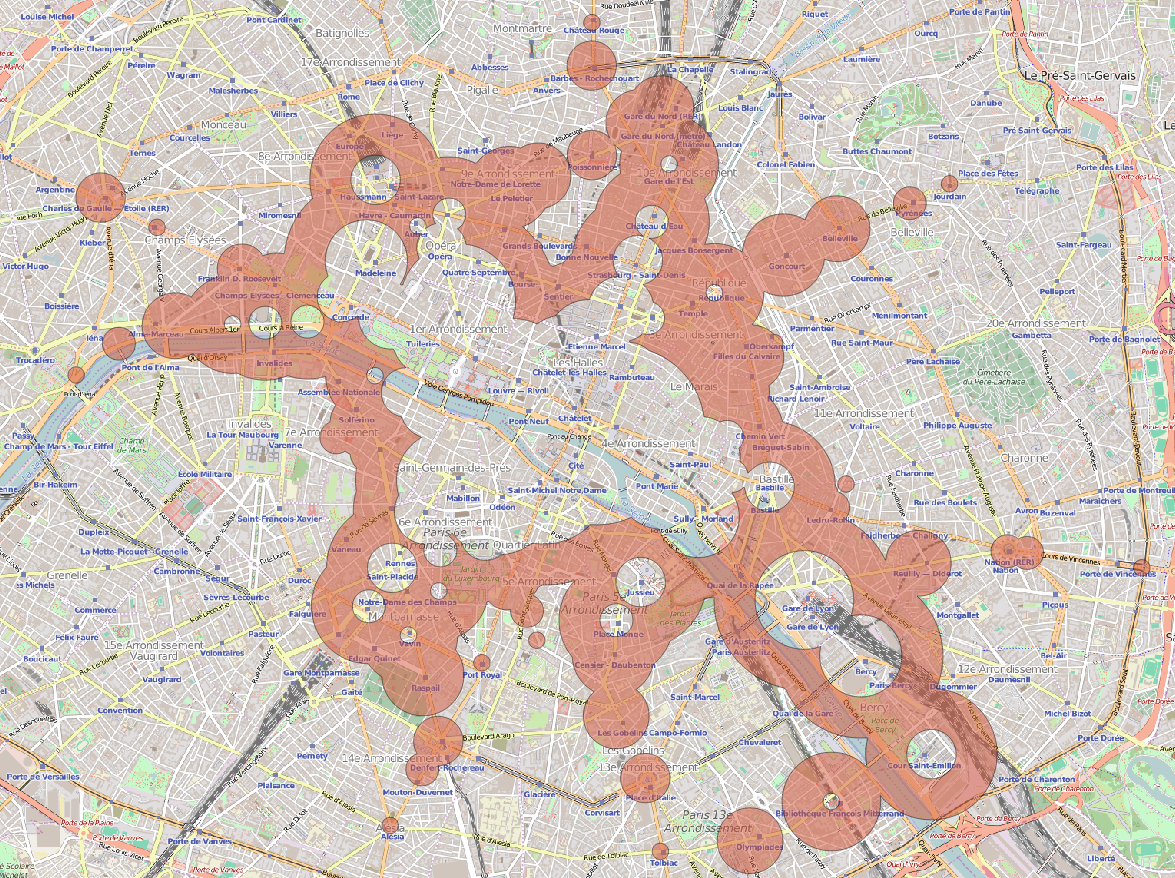
\includegraphics[width=300pt]{image/iso_min}
		\caption{Isochrone entre deux durées}
		\label{Isochrone entre deux durées}
	\end{center}	
\end{figure}

\paragraph{} La réponse de l'API \emph{isochrones} est un flux json comportant entre autre un flux geojson qui décrit les multipolygones renvoyés. Le flux prend la forme suivante :


\begin{lstlisting}[language=json,firstnumber=1]
    {
        isochrones :
        [
            0 :
            {
                max_duration : 120,
                from : {...},
                geojson : {...},
                min_duration : 0,
                requested_date_time: "20160718T164045"
            },
            1 : {...},
            2 : {...}
        ],
        feed_publishers :
        [],
        links :
        [
            0 :
            {
                href : "http://localhost:5000/v1/coverage/default/stop_areas/{stop_area.id}",
                type : "stop_area",
                rel : "stop_areas",
                templated : true
            }
        ],
        warnings :
        [
            0 :
            {
                message : "This service is under construction. You can help through github.com/CanalTP/navitia",
                id : "beta_api"
            }]}

\end{lstlisting}

\paragraph{} C'est dans le chanps geojson qu'est stocké l'information géographique. Si on le regarde plus en détail on a un champ de cette forme :


\begin{lstlisting}[language=json,firstnumber=1]

    {
        "geojson":{
            "type":"MultiPolygon",
            "coordinates":[
                [
                    [
                        [
                            2.3186837324,
                            48.9324437042
                        ],
                        [
                            2.3187241561,
                            48.9324771012
                        ],
                        [
                            2.3190737256,
                            48.9327557777
                        ],
                        ["..."],
                        ["..."],
                        ["..."]
                    ]
                ]
            ]
        }
    }
\end{lstlisting}

\paragraph{} Cependant ces dessins d'isochrones ne prennent pas en compte une certain nombre de contraintes physiques inhérentes au territoire où ils sont tracés comme le filaire de voierie ou les cours d'eau. Ainsi un isochrone peut indiquer que l'autre côté de la berge se trouve à moins de 5 min du point de départ demandé alors que le pont pour y acceder se trouve à plus de 10 minutes.

\subsubsection{API heat\_maps} 

\paragraph{} Nous venons de voir que l'API isochrones manquait parfois de précision, c'est pourquoi à la fin de mon stage j'ai fait des recherches sur une autre forme d'isochrones plus précise qui tiendrait compte du filaire de voierie. Pour celà j'ai dû discretiser la zone géographique sur laquelle je calculais l'isochrone. J'ai ainsi obtenu l'API \emph{heat\_maps}.

\begin{figure}[H]
	\begin{minipage}[c]{.46\linewidth}
		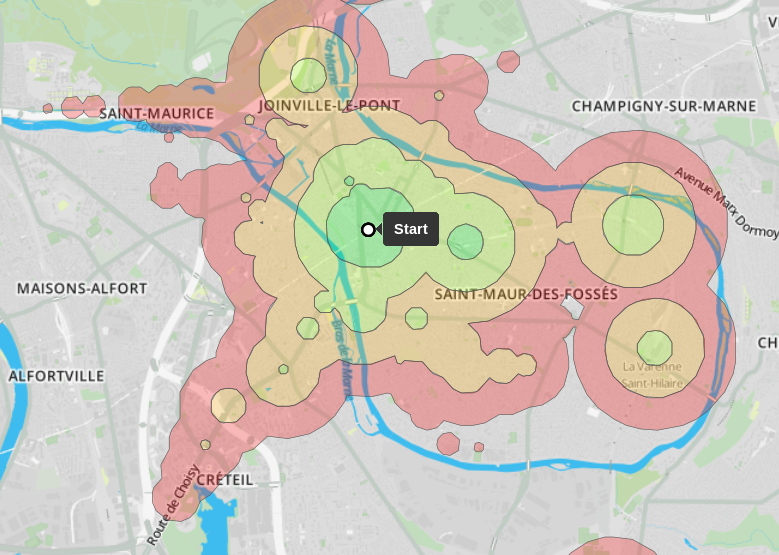
\includegraphics[width=8cm]{image/comp_iso_fin}
       		\caption{Isochrone traversant une rivière}
		\label{Isochrone traversant une rivière}
	\end{minipage} \hfill
	\begin{minipage}[c]{.46\linewidth}
		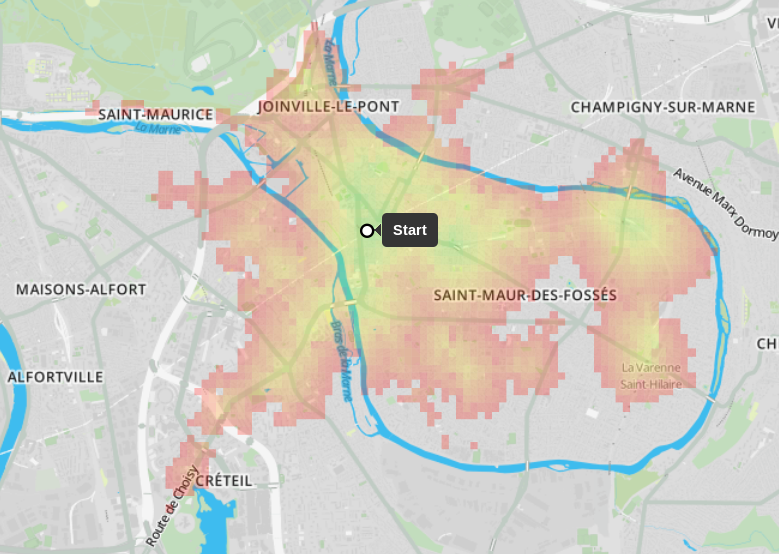
\includegraphics[width=8cm]{image/comp_raster_fin}
       		\caption{Heat map respectant la voierie}
		\label{Heat map respectant la voierie}
	\end{minipage}
\end{figure}

\paragraph{} Cette API est faite pour être plus précise que l'API isochrones, il est donc important de pouvoir définir le degré de discrétisation que l'on souhaite obtenir. Voici ici un exemple où on fait varier le degrè de discrétisation.

\begin{figure}[H]
	\begin{minipage}[c]{.46\linewidth}
		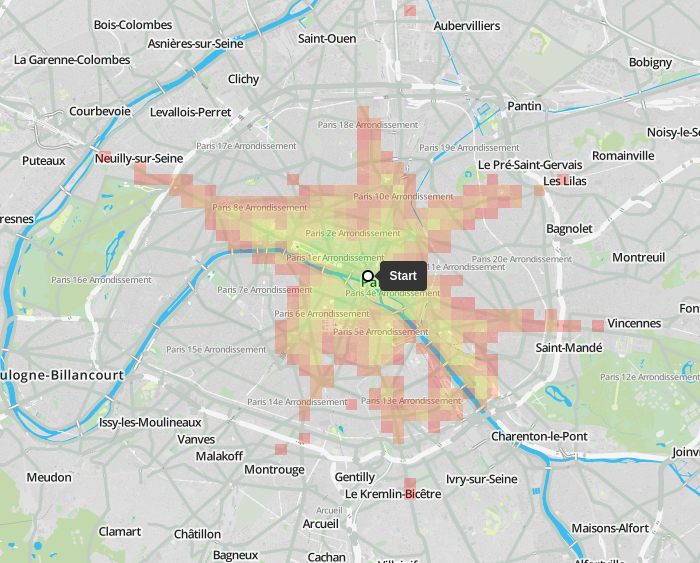
\includegraphics[width=8cm]{image/heatmap_basse_reso}
       		\caption{Heat map resolution = 50}
		\label{Heat map resolution = 50}
	\end{minipage} \hfill
	\begin{minipage}[c]{.46\linewidth}
		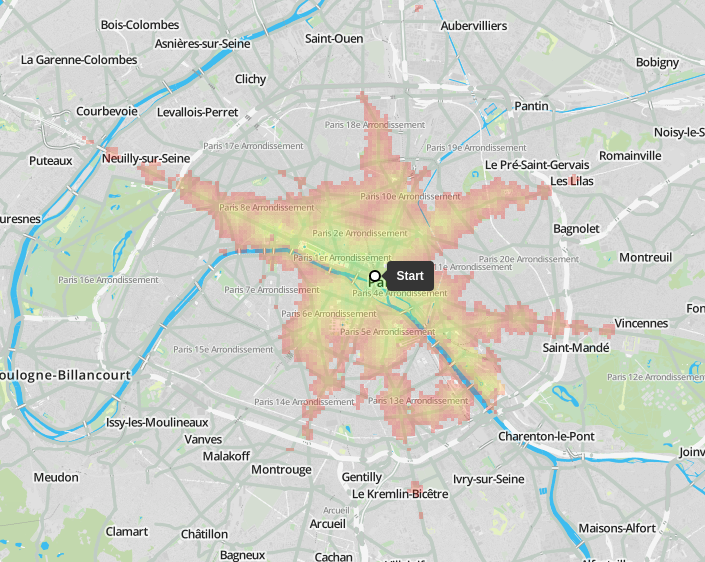
\includegraphics[width=8cm]{image/heatmap_haute_reso}
       		\caption{Heat map resolution = 150}
		\label{Heat map resolution = 150}
	\end{minipage}
\end{figure}

\paragraph{}Cette fois l'API ne renvoit pas uniquement des informations géographiques. L'API doit renseigner les heures d'arrivées au plus tôt (ou les heure de départ au plus tard si on calcule un isochrone inverse) de tous les éléments discrétisés, elle doit également contenir les informations géograhiques permettant de géolocaliser chacun de ces éléments. De plus, le flux json renvoyé doit être le plus petit possible, il ne faut donc pas avoir d'information redondante. Le flux renvoyé est le suivant :

\begin{lstlisting}[language=json,firstnumber=1]
    {
        heat_maps :
        [
            0 :
            {
                requested_date_time : "20160718T164045",
                from : {...},
                heat_matrix : {...}
            }
        ],
        links :
        [
            0 :
            {
                href : "http://localhost:5000/v1/coverage/default/stop_areas/{stop_area.id}",
                type : "stop_area",
                rel : "stop_areas",
                templated : true
            }
        ],
        warnings :
        [
            0 :
            {
                message : "This service is under construction. You can help through github.com/CanalTP/navitia",
                id : "beta_api"
            }
        ]
    }
\end{lstlisting}

\paragraph{} Les informations sont regroupées dans le champs heat\_matrix qui est de la forme suivante :

\begin{lstlisting}[language=json,firstnumber=1]
    heat_matrix :
    {
        line_headers :
        [
            0 :
            {
                cell_lat :
                {
                    min_lat : 48.7971,
                    max_lat : 48.7996,
                    center_lat : 48.7984
                }
            },
            1 : {...},
            2 : {...},
            3 : {...},
        ],
        lines :
        [
            0 :
            {
                duration :
                [
                    0 : 1159,
                    1 : null,
                    2 : 1047,
                    3 : 1035
                ],
                cell_lon :
                {
                    min_lon : 2.36887,
                    center_lon : 2.37088,
                    max_lon : 2.3729
                }
            },
            1 : {...},
            2 : {...},
            3 : {...},
        ]
    }
\end{lstlisting}

\paragraph{} Pour dessiner les heat maps il faut allouer une couleur à chaque durée puis parcourir les objets correspondants au champ \emph{lines}. grâce au champ \emph{cell\_lon} on peut avoir la longitude de la cellule à colorer. Pour obtenir sa latitude il faut faire correspondre chaque objet du tableau dans le champ \emph{duration} à l'objet de même indice dans \emph{line\_headers}. Dans l'exemple précédent par exemple la cellule dont la longitude est comprise entre 2.36887 et 2.3729 et dont la latitude est entre 48.7971 et 48.7984 correspond à un temps d'accès de 1159 secondes.

\section{Algorithmie}

\paragraph{} Les deux APIs présentées dans ce rapport reposent sur des algorithmes très différents. Le but de cette partie est de présenter sommairement le raisonnement sur lequel elles reposent et d'expliquer les difficultés rencontrées. Le code détaillé est disponnible sur \color{blue} https://github.com/CanalTP/navitia. 

\color{black}
\paragraph{}L'algorithme RAPTOR de Navitia possède une fonction isochrone. Celle-ci renvoit un tableau de tous les points d'arrêt avec leurs temps d'accès atteignables à partir du point de départ dans l'horizon de temps donné. Je suis partie de ce tableau pour créer les deux APIs \emph{isochrones} et \emph{heat\_maps}.

\subsection{Pseudo code}

\paragraph{isochrones :} Cette API consiste à tracer des cercles autour des points d'arrêt atteignables.
\newline

\begin{algorithm}[H]
 \KwData{isochrones de RAPTOR, point de départ, durée de l'isochrone}
 \KwResult{multipolygone sous forme de geojson }
 initialiser l'isochrone avec un cercle autour du point de départ en fonction de la durée de l'isochrone\;
 \For{tous les points d'arrêt dans l'isochrone de raptor}{
  \If{temps d'accès < durée maximale}{
   calculer temps restant\;
   tracer un cercle dont le rayon dépend du temps restant\;
    fusionner le cercle avec le multipolygone\;
 }
 }
 \caption{Algorithme de l'API isochrones}
\end{algorithm}

\paragraph{heat\_maps :} Cette API est basée sur l'algorithme de Dijkstra. Cet algorithme permet de résoudre les problèmes de plus court chemin dans un graphe. En appliquant l'algorithme de Dijksta au filaire de voierie on peut donc déterminer le temps d'accès minium pour accéder à chaque noeud de la voierie en partant d'un point donné. Pour l'API heat\_maps nous avons besoin d'utiliser un algorithme de Dijkstra un peu particulier car nous ne donnons pas un seul point de départ. En effet l'algorithme de Dijkstra parcourt le graphe toujours à la même "vitesse". Donc pour prendre en compte les différents modes de transport, il faut donner plusieurs points de départ, avec des dates de départs différentes, à l'algorithme de Dijkstra. Par la suite nous appellerons cette algorithme Dijksta\_multi\_start.
\newline

\begin{algorithm}[H]
 \KwData{isochrones de RAPTOR, point de départ, durée de l'isochrone, résolution de la grille, filaire de voierie}
 \KwResult{tableau de durée et de coordonnées géograhiques}
 \For{tous les points d'arrêt dans l'isochrone de raptor}{
initialiser Dijksta\_multi\_start \;
 }
 lancer Dijksta\_multi\_start \;
 tracer la grille\:
 \For{chaque cellule de la grille}{
 projeter le centre de la cellule sur le filaire de voierie \;
 récupérer le temps d'accés calculé par Dijksta\_multi\_start pour le noeud du graphe le plus proche\;
 remplir le tableau pour la cellule\;
 }
 \caption{Algorithme de l'API heat\_maps}
\end{algorithm}

\subsection{La géométrie sphérique}

\begin{wrapfigure}[13]{r}{5cm}
		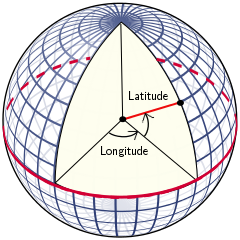
\includegraphics[width=4cm]{image/lat_lon}
		\caption{Coordonnées à la surface de la Terre}
		\label{Coordonnées à la surface de la Terre}
\end{wrapfigure}

\paragraph{} Pour les deux APIs, j'ai eu besoin d'outils géométriques afin de tracer les isochrones. Navitia doit pouvoir être utilisé quelque soit l'endroit où on se trouve sur la Terre. Il est donc impossible de faire des approximations locales permettant de raisonner en géométrie euclidienne. J'ai donc dû utiliser de la géométrie sphérique.

\paragraph{} La géométrie sphérique est la géométrie utilisée sur une surface sphérique. Elle diffère de la géométrie euclidienne pour laquelle la surface de base est un plan. En géométrie sphérique deux droites parallèles peuvent se couper sans être confondues et la somme des angles d'un triangle est suppérieure à l'angle plat. Beaucoup de définitions géométriques doivent donc être redéfinies. Pour ce type de géométrie on n'utilise plus les coordonées cartésiennes mais les coordonnées sphériques. Dans le cas de la terre on appelle ces coordonnées latitude et longitude. Dans la suite de ce rapport la longitude sera notée $\lambda$ et la latitude $\theta$, les longueurs seront exprimées en mètres et les angles en radians.

\subsubsection{Faire une grille sur une sphère}

\paragraph{} Pour créer l'API heat\_maps j'ai eu besoin de diviser la zone que j'étudiais en une grille. Pour cela j'ai utilisé des paralléles et des méridiens de la sphère terrestre. ces lignes délimitent de petites zones qui en géométrie euclidienne seraient équivalentes à des rectangles. Cette méthode est très simple à intégrer mais ne garantit pas la même précision selon l'endroit du globe où est calculé l'isochrone. Ainsi plus on se raprochera d'un pôle, plus l'air d'une cellule sera faible et donc plus la précision augmentera.

\begin{figure}[H]
	\begin{center}
		
\includegraphics[width=200pt]{image/grille_sphere}
		\caption{Grille à la surface d'une sphère}
		\label{Grille à la surface d'une sphère}
	\end{center}
\end{figure}

\subsubsection{Tracer un cercle à la surface d'une sphère}

\begin{wrapfigure}[15]{r}{5cm}
		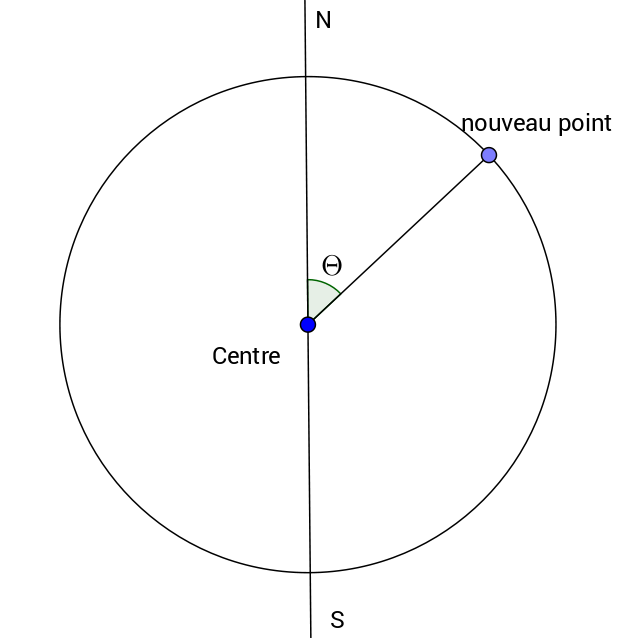
\includegraphics[width=5cm]{image/proj}
		\caption{point projeté}
		\label{point projeté}
\end{wrapfigure}

\paragraph{} Comme nous l'avons vu précédemment l'algorithme de l'API isochrones consiste essentiellement à tracer des cercles autour de points précis. Si on revient à la définition d'un cercle on peut dire que c'est l'ensemble de points à une distance constante que nous appellerons \emph{rayon} d'un point donné que nous appellerons \emph{centre}.

\paragraph{} Le geojson est un format qui permet de caractériser des polygones comportant un nombre fini de points, il est donc impossible de tracer un cercle parfait qui est un ensemble infini de points. Il faut discrétiser le cercle. Pour que les points soient uniformément répartis il faut échantillonner le cercle en fonction de l'angle au centre. Cela permet également de facilement choisir le nombre de points et donc la précision qui sera nécessaire à la cartographie sans trop alourdir le flux. La première chose à savoir faire est donc être capable de déterminer les coordonnées sphériques d'un point à une distance donnée d'un centre et avec un angle au centre donné. L'angle au centre est arbitrairement choisit comme étant l'angle entre le segment du méridien passant par le centre et le segment reliant le point projeté et le centre, sur le schéma ci-contre il est noté $\theta$.

\subsection{Résolutions mathématiques}

\paragraph{} Pour implémenter la fonction que nous venons de décrire, il est nécessaire d'avoir quelques notions de géométrie sphérique. Nous avons donc utilisé la trigonométrie sphérique, qui permet d'établir des liens entre les distances et les angles, pour résoudre ce problème. Nous présentons ici les relations qui nous seront utiles dans un triangle rectangle sphérique.

\paragraph{} En géométrie sphérique un triangle est une surface délimitée par des arcs de grands cercles. Un triangle rectangle sphérique est un rectangle dont l'un des angles mesurent $\frac{\pi}{2}$ rad. Il est toutefois important de noter que la somme des angles d'un tel triangle est suppérieure à $\pi$ et que les relations de trigonométrie euclidienne ne sont pas valides ici. A la place on utilise les relations suivantes :

\begin{figure}[H]
	\begin{minipage}[c]{.46\linewidth}
		\begin{center}
			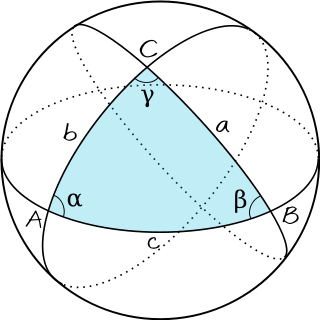
\includegraphics[width=5cm]{image/sprint2_triangles_spheriques}
       			\caption{Triangle rectangle spérique}
			\label{Triangle rectangle spérique}
		\end{center}
	\end{minipage} \hfill
	\begin{minipage}[c]{.46\linewidth}
		\begin{align}
			\sin(a)&=\sin(c)\sin(\alpha) \\
			\cos(c)&=\cos(b)\cos(a) 
		\end{align}
	\end{minipage}
\end{figure}

\paragraph{} Grâce à ses propriétés nous pouvons maintenant procéder à la résolution mathématiques. Supposons que le point P de coordonnées ($\theta_{0}$, $\lambda_{0}$) soit le centre du cercle que nous souhaitons tracer. On nommera respectivement $\lambda$ et $\theta$ la longitude et la latitude du point projeté formant un angle $\phi$ avec le méridien passant par P. Le rayon du cercle est $d$ et $\alpha$ correspond à l'ouverture d'angle entre P et le nouveau point. Enfin $R$ est le rayon de la Terre.

\paragraph{} On modélise notre problème grâce aux figures suivantes :

\begin{figure}[H]
	\begin{center}
		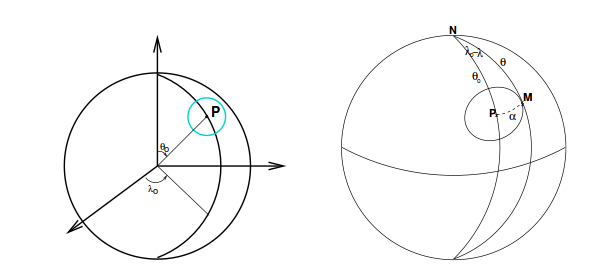
\includegraphics[width=400pt]{image/sprint2_petits-cercles}
		\caption{Cercle à la surface d'une sphere}
		\label{Cercle à la surface d'une sphere}
	\end{center}
\end{figure}

\paragraph{} On peut donc facilement en déduire une relation entre $d$, $\alpha$ et $R$ :

\begin{figure}[H]
	\begin{minipage}[c]{.46\linewidth}
		\begin{center}
			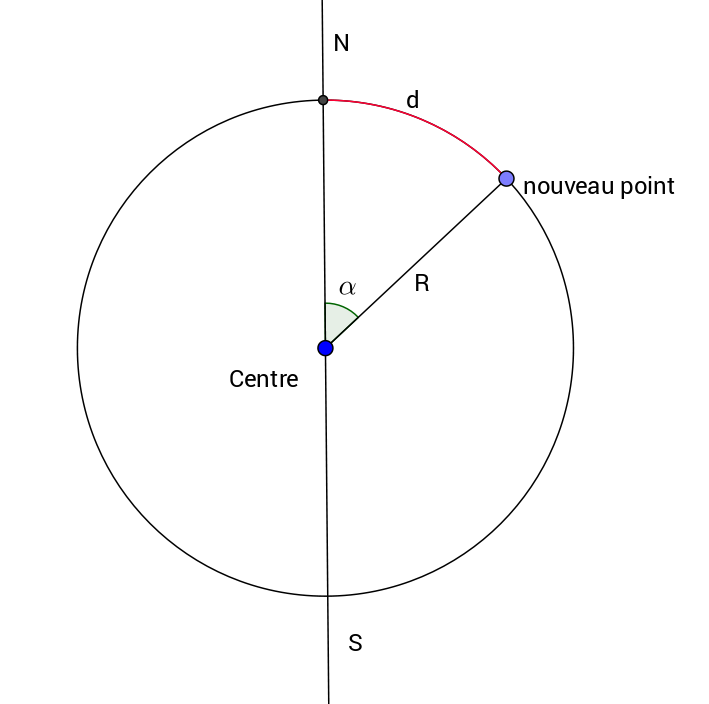
\includegraphics[width=6cm]{image/relation_angle_rayon}
       			\caption{Relation rayon ouverture d'angle}
			\label{Relation rayon ouverture d'angle}
		\end{center}
	\end{minipage} \hfill
	\begin{minipage}[c]{.46\linewidth}
		\begin{align}
			\alpha &= \frac{d}{R}
		\end{align}
	\end{minipage}
\end{figure}	

\paragraph{} Par ailleurs on sait que l'équation d'un cercle sur une sphère est l'ensemble des points de coordonnées $\theta$ et $\lambda$ tel que \cite{ref_cercle_sphere}:
\begin{align}
	\cos\alpha &= \cos\theta\cos\theta_{0} + \sin\theta\sin\theta_{0}\cos(\lambda - \lambda_{0})
\end{align}

\paragraph{} En mettant en commun toutes ces équations on obtient donc le système d'équation suivant :

\begin{align} 
	p&=\arcsin(\sin(\alpha)\sin(\phi)) \\
	\Delta \theta &= 
	\left \{
	\begin{array}{r c l}
		\arccos(\frac{\cos(\alpha)}{\cos(p)}) \quad si& \phi \ge 0 \\
		-\arccos(\frac{\cos(\alpha)}{\cos(p)}) \quad si& \phi < 0\\
	\end{array}
	\right. \\
	\theta &= \theta_{0} + \Delta \theta \\
	\Delta \lambda &= 
	\left \{
	\begin{array}{r c l}
		\arccos(\frac{\cos(\alpha) - \sin(\theta)\sin(\theta_0)}{\cos(\theta)\cos(\theta_0)}) \quad si& \phi \in \left[ -\frac{\pi}{2},\frac{\pi}{2} \right]\\
		-\arccos(\frac{\cos(\alpha) - \sin(\theta)\sin(\theta_0)}{\cos(\theta)\cos(\theta_0)}) \quad si& \phi \in \left] \frac{\pi}{2},\frac{3\pi}{2} \right]\\
	\end{array}
	\right. \\
	\lambda &= \lambda_{0} + \Delta \lambda 
\end{align}

\paragraph{} Il suffit ensuite de faire varier $\phi$ entre $\left[ 0, 2\pi \right]$ avec un pas constant pour obtenir un ensemble de points qui correspondra au cercle discrétisé que nous souhaitons tracer.

\section{Les performances}

\paragraph{}Pour que l'API soit efficace il était nécessaire que ses performances permettent de travailler avec des grands jeux de données. A titre d'exemple : l'Ile de France comporte plus de 40 000 points d'arrêt. Optimiser le temps de réponse de Navitia était donc un enjeu majeur de mon stage. Dans cette partie nous verrons les diférents moyens utilisés pour optimiser le temps de réponse de l'API isochrones et heat\_maps. 

\paragraph{}Le logiciel Navitia est paramétré de façon à ce que Jormungandr renvoie un message d'erreur si le temps de calcul dans Kraken dépasse 10 secondes. Il a donc fallu prendre en compte cette contrainte pour rendre les deux APIs opérationnelles. Dans la suite de cette partie, toutes les courbes représentées feront référence à l'API isochrones qui a bénéficié d'une plus longue étude de ses performances.

\subsection{Méthodologie}

\paragraph{} Pour étudier les performances dans Kraken il fallait savoir combien de temps le programme passait dans chaque fonction. L'outil \emph{google CPU profiler} permet d'identifier les morceaux de codes où le programme passe le plus de temps. 

\begin{figure}[H]
	\begin{center}
		\includegraphics[width=300pt]{image/profile_with_simplify}
		\caption{Interface de google CPU profiler}
		\label{Interface de google CPU profiler}
	\end{center}
\end{figure}

\paragraph{} \emph{Google CPU profiler} permet d'estimer le nombre d'appels fait à chaque fonction ainsi que le pourcentage de temps passé dans chaque fonction. Pour avoir une estimation fiable de ces données on a utilisé un script \emph{shell} permettant de faire une centaine d'appels de façon automatique aux APIs isochrones et heat\_maps. On peut ainsi identifier les fonctions les plus coûteuses en temps. Cette méthode permet d'identifier les fonctions à optimiser en priorité. 

\paragraph{} En une requète on peut demander au plus 10 isochrones. Il faut donc que le temps de réponse pour un isochrone soit de l'ordre de $0.5$ seconde et ce quelque soit la durée et l'emplacement de l'isochrone. Nous avons estimé que si cette condition était satsifaite à 8h00 du matin à la station Châtelet alors l'API pouvait passer en production. Avant toute optimisation on avait les temps de réponse suivants :

\begin{figure}[H]
	\begin{center}
		\includegraphics[width=400pt]{image/avant_opt}
		\caption{Profil de temps de réponse avant optimisation pour l'API isochrones}
		\label{Profils de temps de réponse avant optimisation pour l'API isochrones}
	\end{center}
\end{figure}

\subsection{Influence du tri}

\paragraph{}Comme nous l'avons dit précédemment le réseau de transport en commun de l'Ile de France comporte plus de 40 000 points d'arrêt. Pour de grandes durées le nombre de points d'arrêt contenus dans un isochrone est donc très important. Or dans l'algorithme utilisé le temps de réponse dépend du nombre de polygones dans le multipolygone qui représente l'isochrone. Il faut donc avoir le moins de polygones possible dans le multipolygone. C'est pourquoi, à chaque fois qu'on ajoute un cercle on essaye de le faire fusionner avec les polygones déjà existants. 

\paragraph{} Lorsque les points d'arrêt sont pris dans un ordre aléatoire on a la courbe suivante pour un isochrone partant de Châtelet à 8h00 et ayant une durée d'une heure. Chaque itération correspond à la prise en compte d'un nouveau point d'arrêt.

\begin{figure}[H]
	\begin{center}
		\includegraphics[width=400pt]{image/nb_poly_avt_opt}
		\caption{Nombre de polygones pour un ordre aléatoire}
		\label{Nombre de polygones pour un ordre aléatoire}
	\end{center}
\end{figure}

\paragraph{} On observe que le nombre de polygones augmente très rapidement. Maintenant si on pense à trier les cercles en fonction de la distance qui les sépare du centre de l'isochrone, en prenant d'abord en compte les cercles les plus proches du centre, on peut supposer que les polygones seront plus souvent adjacents et donc qu'on pourra aisément les faire fusionner entre eux, ce qui minimisera leur nombre. 

\paragraph{} Lorsqu'on trie les points d'arrêt en fonction de leur proximité avec le point de départ de l'isochrone on obtient la courbe suivante :

\begin{figure}[H]
	\begin{center}
		\includegraphics[width=400pt]{image/nb_poly_ap_opt}
		\caption{Nombre de polygones lorsqu'on ordonne les points d'arrêt}
		\label{Nombre de polygones lorsqu'on ordonne les points d'arrêt}
	\end{center}
\end{figure}

\paragraph{} Le nombre de polygones n'augmente qu'à partir des dernières itérations, ce qui minimise considérablement les calculs faits pendant les itérations précédentes et contribue à améliorer les temps de calcul dans Kraken.

\subsection{Echantillonnage}

\paragraph{} Nous l'avons vu, le calcul des coordonnées d'un cercle sur une sphère est fastidieux et fait appel à des fonctions trigonométriques. Or ces fonctions sont coûteuses en temps, il faut donc les appeler un minimum de fois. Pour celà il est judicieux d'exploiter les nombreuses symétries du cercles. En effet on peut calculer toutes les coordonnées d'un quart de cercle puis utiliser ses symétries par rapport à l'axe des abscisses et des ordonnées d'un repère polaire afin de reconstruire le cercle en entier. Cette opération est d'autant plus facile que ces symétries sont les mêmes qu'en géométrie euclidienne. Cette méthode permet de ne plus appeler les fonctions construisant un point d'un cercle qu'une fois là où elles étaient auparavant appelées quatre fois.

\paragraph{} D'autre part, nous avons déjà vu que les cercles que nous traçions étaient en réalité des cercles échantillonés. Initialement ces polygones possédaient 360 points. En divisant ce nombre par deux, on réduit par deux le nombre d'appels aux fonctions trigonométriques utilisées ce qui permet là encore d'améliorer le temps de réponse de l'API.

\paragraph{} Après toutes les optimisations que nous venons de décrire nous pouvons tracer la courbe bleue qui représente les nouveaux temps de réponse :

\begin{figure}[H]
	\begin{center}
		\includegraphics[width=300pt]{image/nvx_tmps}
		\caption{En rouge: temps de réponse avant tri et rééchantillonage, en bleu : temps de réponse après}
		\label{Temps de réponse après tri et rééchantillonnage}
	\end{center}
\end{figure}

\paragraph{} Enfin le rééchantillonage des polygones a également permis de réduire de moitié la taille des flux que l'API isochrones donnait en réponse.

\begin{figure}[H]
	\begin{center}
		\includegraphics[width=300pt]{image/taille_flux}
		\caption{En rouge: taille du flux avant tri et rééchantillonage, en bleu : taille du flux après}
		\label{Taille du flux après tri et rééchantillonnage}
	\end{center}
\end{figure}

\paragraph{} Dans l'API heat\_maps la taille de la grille utilisée influe également sur le temps de calcul et la taille du flux de sortie. Pour que le temps de calcul n'excède pas $10$ secondes le nombre de pixels sur une ligne de la grille qui divise la zone d'étude ne peut pas dépasser $1000$.

\subsection{Distance et projection}

\paragraph{} Les fonctions trigonométriques sont des fonctions qui demandent un temps de calcul important, il est donc capital de les utiliser le moins possible si on veut améliorer le temps de calcul. Cependant pour les APIs isochrones et heat\_maps nous avons souvent besoin d'utiliser des fonctions permettant d'évaluer des distances entre deux points d'une sphère. Pour cela on utilise la formule d'Haversine :

\begin{align}
	d &= 2r\arcsin\left(\sqrt{\sin^2\left(\frac{\theta_{2} - \theta_{1}}{2}\right)+\cos\theta_{1}\cos\theta_{2}\sin^2\left(\frac{\lambda_{2} - \lambda_{1}}{2}\right)}\right)
\end{align}

\paragraph{} Où d est la distance entre les deux points de coordonnées ($\theta_{1}$, $\lambda_{1}$) et ($\theta_{2}$, $\lambda_{2}$).

\paragraph{} Cette formule comporte ce nombreuses fonctions trigonométriques. Or la plupart du temps dans l'algorithme, ce n'est pas la distance en elle-même qui importe mais la possibilité de comparer deux distances entre elles. De plus sur des distances inférieures à une centaine de kilomètre le biais introduit par la courbure de la Terre peut être négligé. On utilise alors une autre formule pour calculer les distances.

\begin{align}
	d &= \sqrt{r^2\left(\theta_{2} - \theta_{1}\right)+\left(\lambda_{2} - \lambda_{1}\right)\cos\theta_{1}}
\end{align}

\paragraph{} Cette nouvelle fonction permettant de calculer les distances est utilisée dans l'API isochrones afin d'ordonner les points d'arrêt et de calculer le rayon des cercles à tracer autour d'eux. Elle est aussi utilisée dans l'API heat\_maps où elle permet de projeter les centres des pixels de la grille d'échantillonnage sur les arcs du graphe du filaire de voierie. Dans les deux cas cette formule abaisse significativement le temps de calcul dans Kraken. 

\begin{figure}[H]
	\begin{center}
		\includegraphics[width=400pt]{image/derniere_opt}
		\caption{En rouge: temps de réponse avant utilisation de la formule simplifiée, en bleu : temps de réponse après}
		\label{Temps de réponse après utilisation de la formule simplifiée}
	\end{center}
\end{figure}

\paragraph{} Le temps de réponse moyen de l'API isochrones pour un isochrone partant de Châtelet à 8h00 est de $0.39$ secondes.  Pour l'API heat\_maps le temps moyen de calcul est de $3$ secondes. On a donc estimé que les deux APIs pouvaient passer en production.

\section{La visualisation}

\paragraph{} Même si mon stage consistait à retourner des flux json, il était essentiel de pouvoir visualiser ces flux afin de corriger les bugs. Dans un premier temps j'ai utilisé le logiciel qgis en redirigeant les flux json renvoyés par l'API dans un fichier ".txt". Je modifiais ensuite ce fichier à la main afin d'en extraire la partie affichable. Mais cette solution était peu satisaisante, ne fonctionnait pas simplement avec l'API heat\_maps et était trop coûteuse en temps. J'ai donc utilisé deux outils internes de Kisio Digital dans lesquels j'ai codé en javascript des appels aux API isochrones et heat\_maps. Cette partie présente le fonctionnement des deux interfaces homme machine (IHM) utilisées.

\subsection{Navitia Explorer}

\paragraph{} \emph{Navitia Explorer} est l'IHM qui a été utilisée jusqu'en juin 2016 par les dévelopeurs de Kisio Digital. Développée par l'équipe "data" elle permet de visualiser simplement les réponses de Navitia. Son code est disponnible sur \color{blue} https://github.com/CanalTP/navitia-explorer\color{black}. Cette IHM présente les réponses de Navitia sous forme de cartes, de listes et de tableaux afin d'être facilement lisibles.

\begin{figure}[H]
	\begin{center}
		\includegraphics[width=400pt]{image/navexplo_2}
		\caption{Interface de Navitia explorer}
		\label{Interface de Navitia explorer}
	\end{center}
\end{figure}

\paragraph{} Toutes les APIs de Navitia sont accessibles grâce aux onglets situés en haut de la page. Pour accéder à l'API isochrones j'ai donc créé un onglet supplémentaire.

\begin{figure}[H]
	\begin{center}
		\includegraphics[width=400pt]{image/navexplo_iso}
		\caption{Navitia explorer : onglet isochrone}
		\label{Navitia explorer : onglet isochrone}
	\end{center}
\end{figure}

\paragraph{} L'appel à l'API heat\_maps n'a pas été codé dans \emph{Navita explorer} car cette API a été codée après juin 2016. En effet à cette période les dévelopeurs ont commencé à utiliser une nouvelle IHM : \emph{Navitia playground}.


\subsection{Navitia Playground}

\paragraph{} En mai, Kisio Digital a monté une équipe afin d'implémenter une nouvelle IHM permettant de se familiariser avec le fonctionnement de Navitia. Cette équipe à codé en un mois \emph{Navitia playground} dont le code est disponible sur \color{blue} https://github.com/CanalTP/navitia-playground \color{black}. Contrairement à \emph{Navitia explorer}, cette IHM est composée d'une unique page, sans onglets. 

\begin{figure}[H]
	\begin{center}
		\includegraphics[width=400pt]{image/playground_1}
		\caption{page d'accueil de Navitia playground}
		\label{page d'accueil de Navitia playground}
	\end{center}
\end{figure}

\paragraph{} \emph{Navitia playground} permet de voir l'URL qui est utilisée pour interroger Navitia, de plus on a facilement accès au flux json renvoyé par l'API. Cela permet de comprendre plus facilement le fonctionnement du logiciel. En outre le fait d'avoir à la fois le flux json et les informations affichées sous forme de carte permet d'être plus efficace quant à la recherche de bug.

\paragraph{} Quelque soit l'API requétée \emph{Navitia playground} n'a qu'une seule interface qui génère une URL en fonction des paramètres rentrés via l'interface graphique.

\begin{figure}[H]
	\begin{center}
		\includegraphics[width=400pt]{image/playground_2}
		\caption{Page de création de requête}
		\label{Page de création de requête}
	\end{center}
\end{figure}

\paragraph{} Cette structure permet à \emph{Navitia playground} d'avoir un code beaucoup plus factorisé que \emph{Navitia explorer}, il est donc plus facile d'ajouter les réponses des APIs isochrones et heat\_maps dans \emph{Navitia playground} que dans navita explorer. 

\paragraph{} On a donc rapidement intégré les réponses des deux APIs dans \emph{Navitia playground}. La majorité des illustrations de ce rapport viennent de cette IHM.  

\begin{figure}[H]
	\begin{center}
		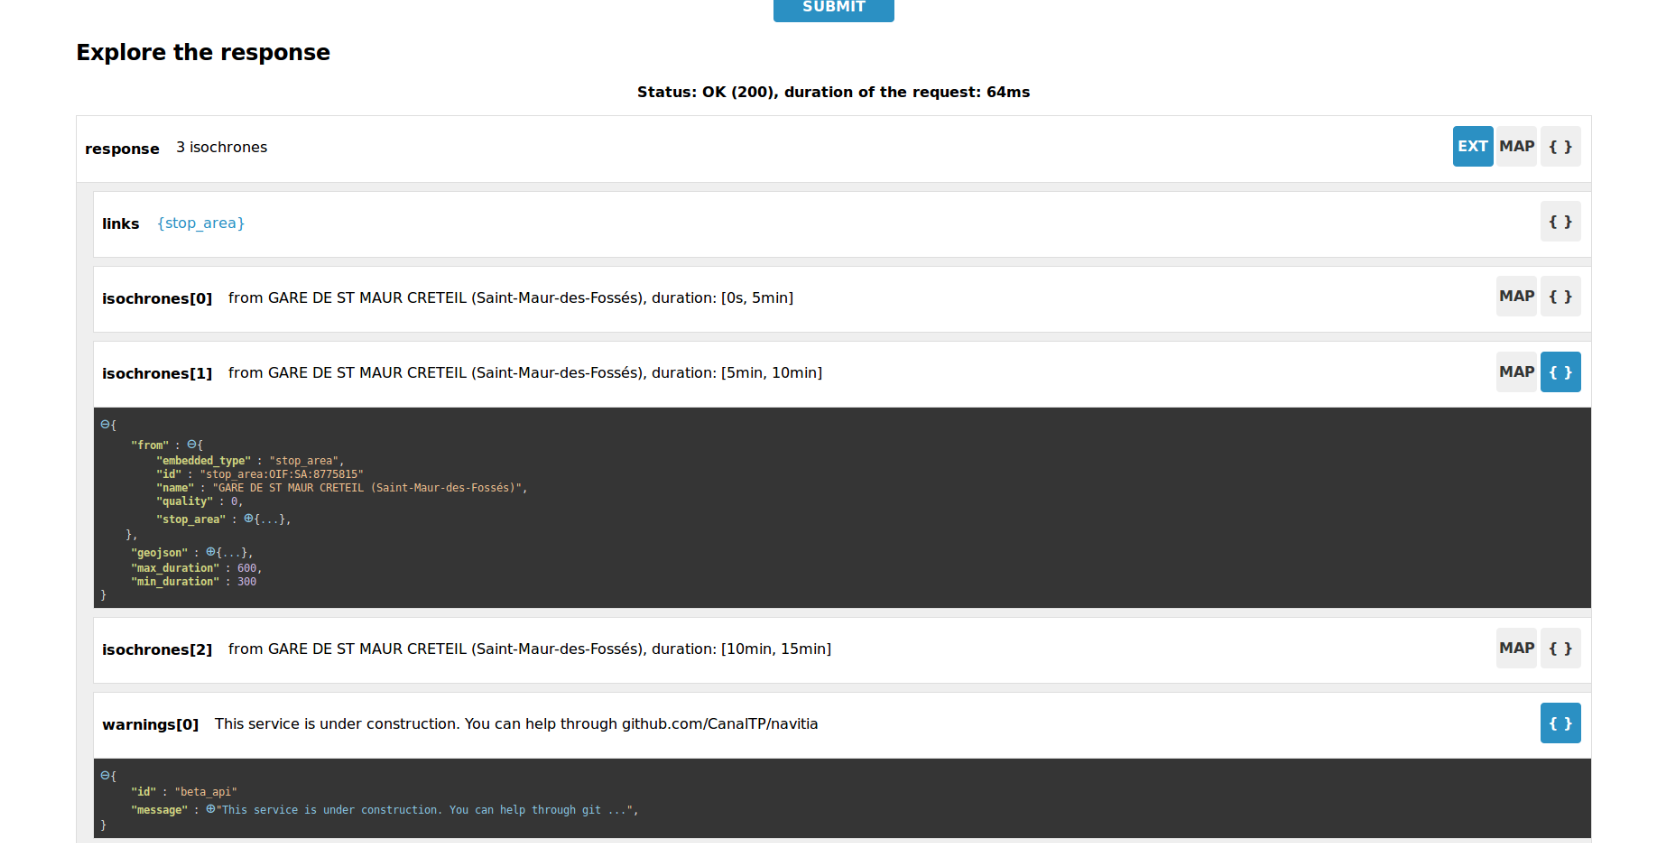
\includegraphics[width=400pt]{image/n_p_flux_json}
		\caption{Navitia playground: requête d'isochrone}
		\label{Navitia playground: requête d'isochrone}
	\end{center}
\end{figure}

\paragraph{} De plus \emph{Navitia playground} permet d'isoler un objet quand plusieurs sont demandés en une seule requête. On peut ainsi choisir d'afficher les objets sur des cartes différentes où sur la même carte en fonction du besoin.

\begin{figure}[H]
	\begin{center}
		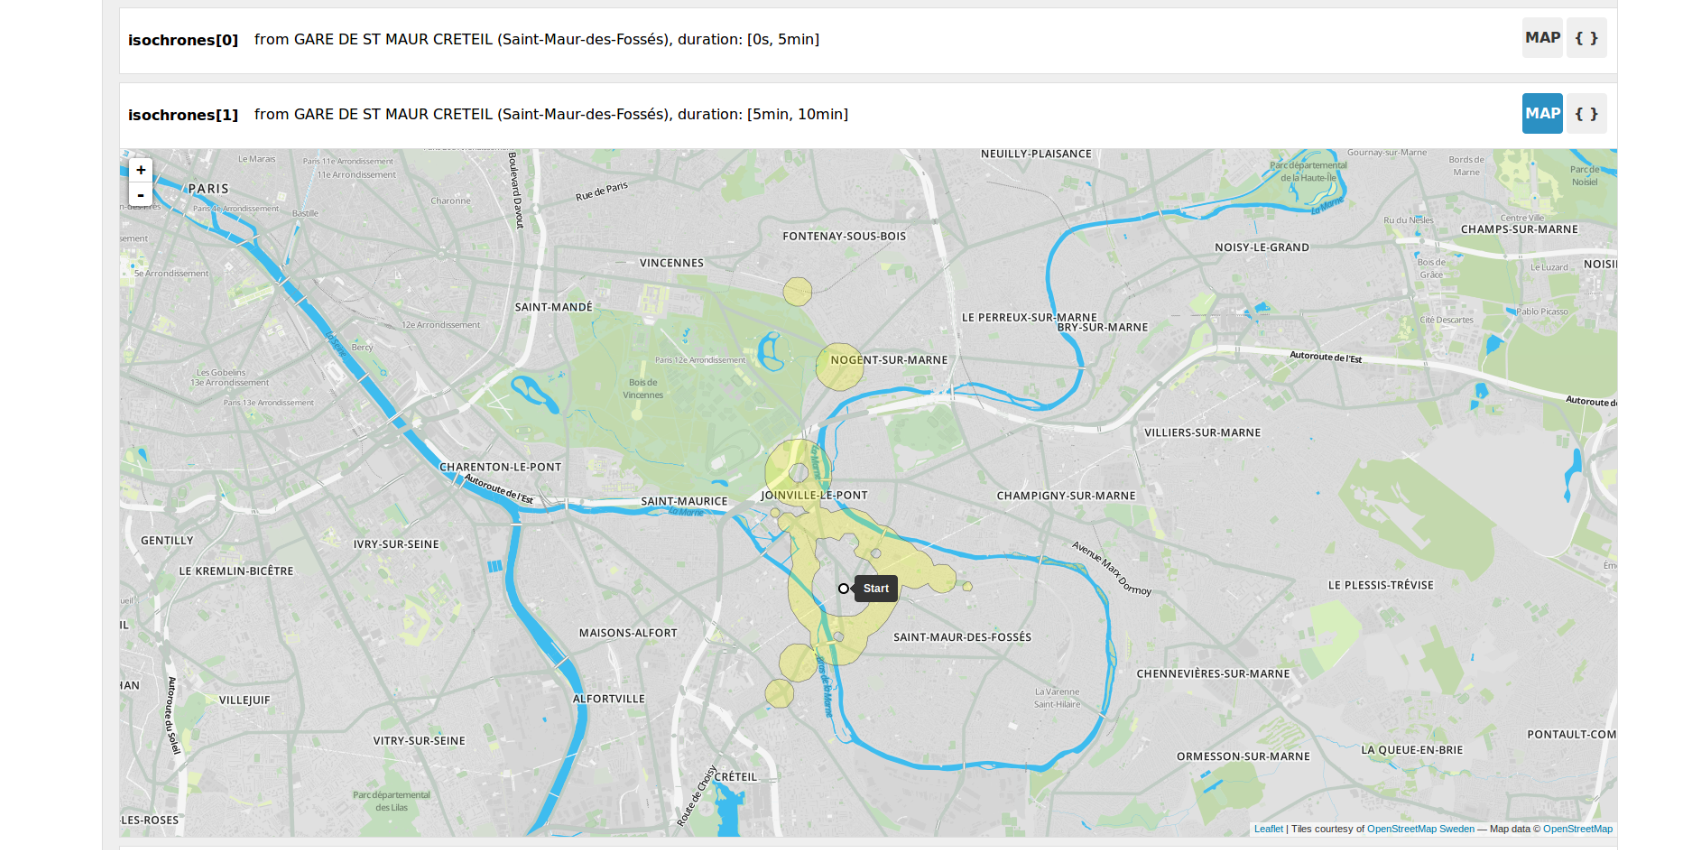
\includegraphics[width=400pt]{image/n_p_iso}
		\caption{Navitia playground: isochrone isolé}
		\label{Navitia playground: isochrone isolé}
	\end{center}
\end{figure}

\begin{figure}[H]
	\begin{center}
		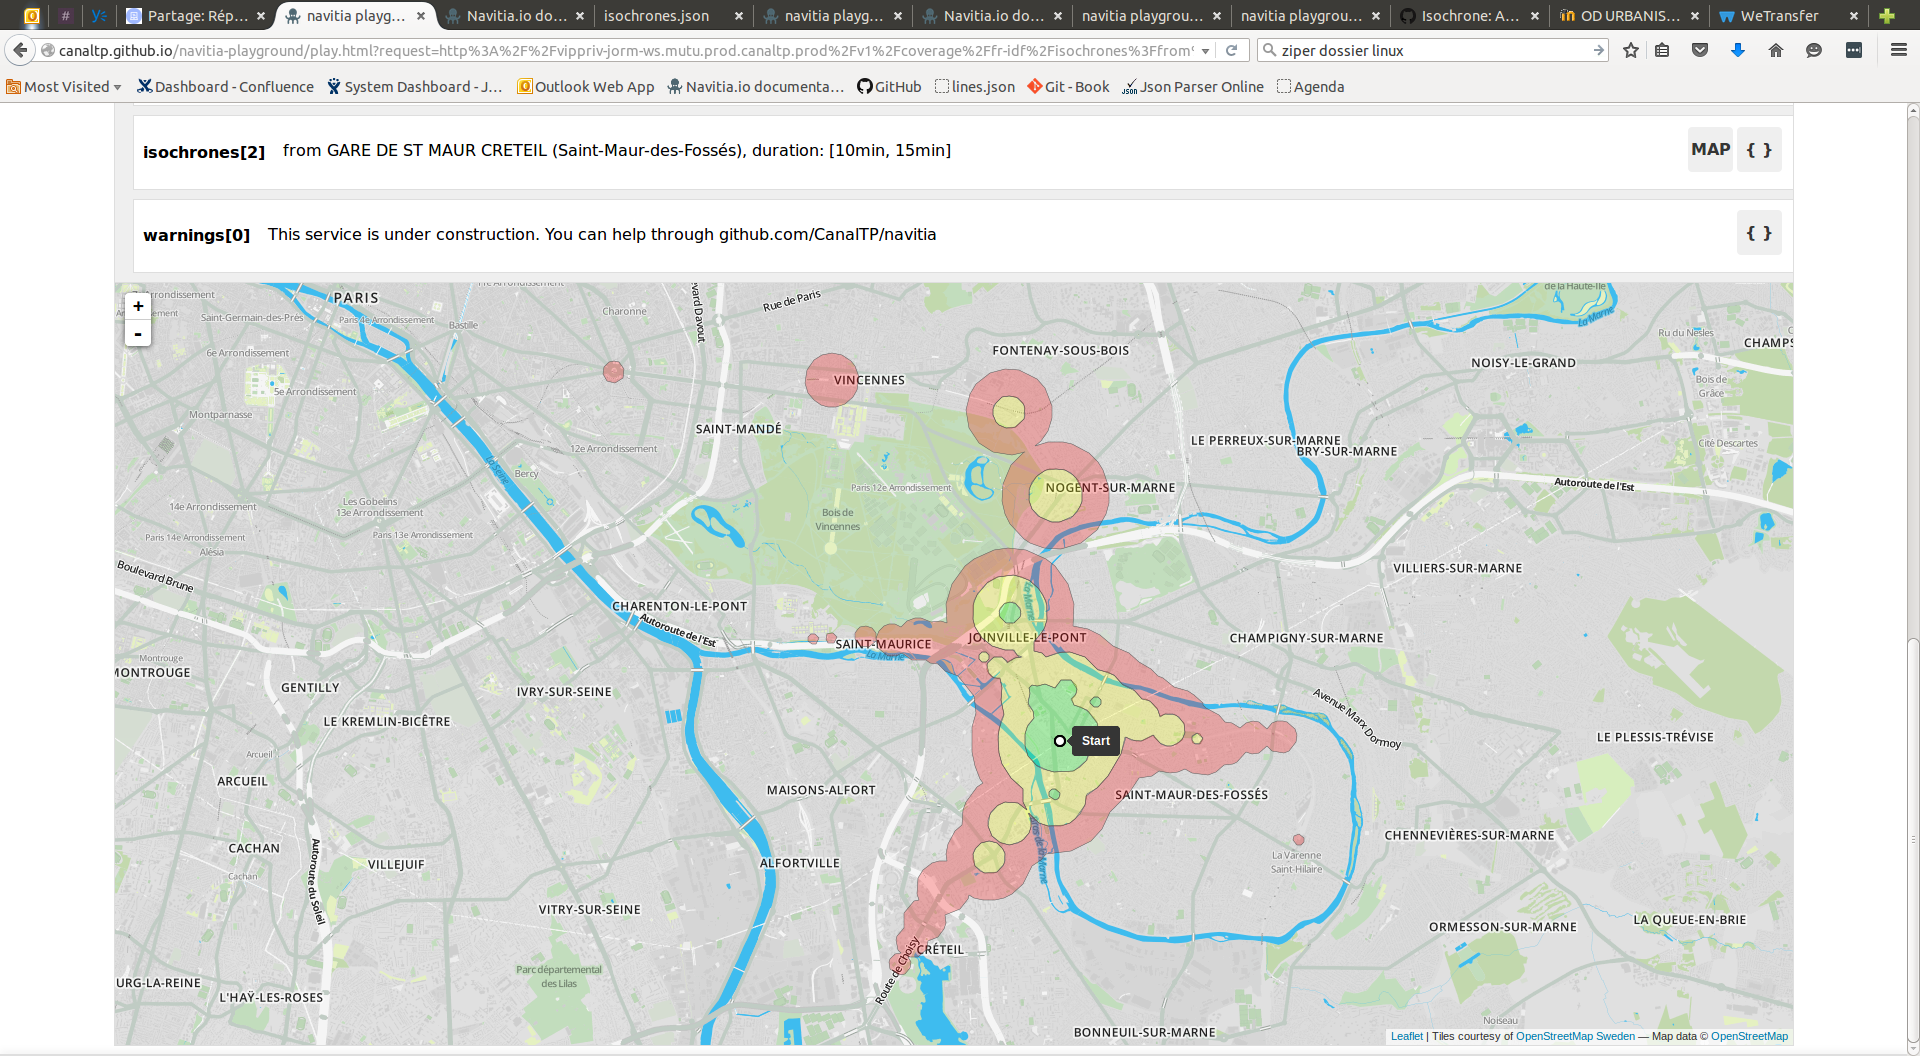
\includegraphics[width=400pt]{image/n_p_isochrone}
		\caption{Navitia playground: isochrones groupés}
		\label{Navitia playground: isochrones groupés}
	\end{center}
\end{figure}

\paragraph{}L'API heat\_maps est aussi affichable dans \emph{Navitia playground}, cependant si la résolution est trop importante, c'est à dire si la grille utilisée pour découper l'espace possède trop de pixels, alors \emph{Navitia playground} ne parvient pas à afficher la heat\_maps car il y a trop de géométries différentes à afficher.

\begin{figure}[H]
	\begin{center}
		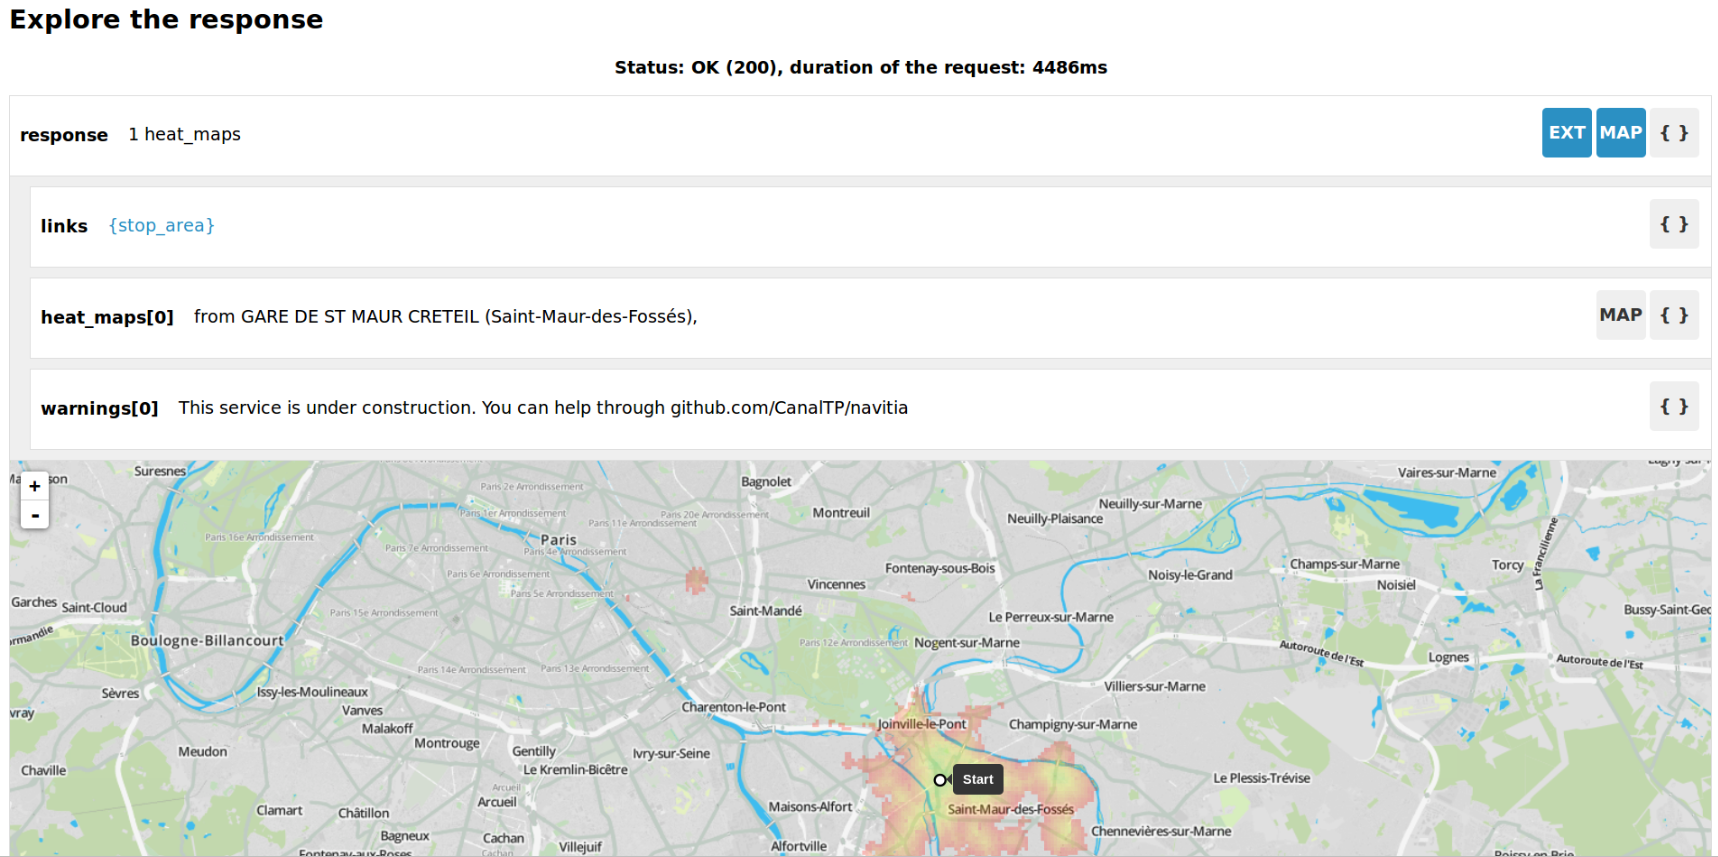
\includegraphics[width=400pt]{image/n_p_heat_map}
		\caption{Navitia playground: requête d'heat maps}
		\label{Navitia playground: requête d'heat maps}
	\end{center}
\end{figure}

\chapter*{Conclusion}
\addcontentsline{toc}{chapter}{Conclusion}

\paragraph{} Ce stage à permis d'implémenter deux APIs dans le logiciel Navitia. Ces deux APIs permettent de représenter des isochrones de façon différente afin de s'adapter au différents usages qui peuvent en être fait. Ces APIs permettent d'avoir des données cartographiques afin de mieux apréhender l'accessibilité au sein des villes en prenant en compte les transports en commun. Le tableau ci-dessous résume les différences entre ces deux APIs\\

\begin{center}
  \begin{tabular} {|l|c|c|}
  \hline
  Critère & Isochrone & Heat map \\
  \hline
  Mode de représentation & vectoriel & raster \\
  \hline
  Temps de réponse & < 1s &  < 3 s \\
  \hline
  Taille du flux & < 1 Mo & 4 Mo \\
  \hline
  Facilement utilisable pour faire des filtres & ++ & + \\
  \hline
   Précision des temps d'accès & + & ++ \\
  \hline
  Prend en compte la voierie à l'arrivée & -- & ++ \\
  \hline
  facilement intégrable & ++ & + \\
  \hline
  \end{tabular}
\end{center}

\paragraph{} Grâce à ce stage, j'ai pu découvrir le travail dans une entreprise d'informatique. Il était particulièrement intéressant d'assister aux changements de méthodes de management qui ont eu lieu au cours de mon stage avec l'arrivée des feature teams. Cela m'a permis de me familiariser avec la méthode Agile et d'être plus à l'aise au sein d'une équipe de dévelopeurs.

\paragraph{} J'ai également acquis des compétences techniques au cours de ce stage. J'ai appris comment développer une API, mais aussi comment la tester et comment optimiser ses performances. De plus j'ai grandement amélioré mes connaissances dans plusieurs langages informatiques comme le C++ et le Python. Sans parler des nombreuses heures dédiées à l'étude des fondamentaux de la géométrie sphérique.

\paragraph{} Enfin j'ai beaucoup apprécié de travailler sur les systèmes d'information voyageurs. Les problématiques qui y sont soulevées m'ont motivée car elles mèlent à la fois des challenges techniques mais aussi des aspects liés à l'utilisateur. Ce qui ne va pas sans me rappeler les objectifs de l'option urbaniSTIC. 

\paragraph{} Ce stage m'a également confortée dans l'idée que je voulais continuer à approfondir mes connaissances en informatique au cours de mes études. J'ai beaucoup aimé travailler dans une équipe de recherche opérationnelle et j'aimerais continuer sur cette voie en faisant des études me permettant de faire de la recherche.

\chapter*{Glossaire}
\addcontentsline{toc}{chapter}{Glossaire}

\begin{description}
	\item[API:] Interface de programmation applicative ou Application Programming Interface
	\item[Editeur Saas:] Logiciel en tant que service ou software as a service. Modèle d'exploitation commerciale des logiciels dans lequel ceux-ci sont installés sur des serveurs distants plutôt que sur la machine de l'utilisateur.
	\item[ESB :] Concept central d'une architecture SOA. Se connecte aux briques métiers pour fournir les services spécifiques.
	\item[ETL :] Connecteur aux données métier. Transforme les donnés d'un format vers un autre.
	\item[GeoJSON:] Json géographique
	\item[IHM: ] Interface Homme Machine
	\item[Json:] JavaScript Object Notation
	\item[MDM :] Standardisation des données. Agrégation : traitement des données dupliquées / dédoublées / enrichissement
	\item[SAEIV:] Systèmes d'Aides à l'Exploitations et Informations Voyageurs 
	\item[SIV :] Système d'Information Voyageur.
	\item[SOA :] Concept d'une architecture orientée service. Organiser de manière homogène les traitements métiers déportés dans des services spécifiques.
\end{description} 

\appendix
\listoffigures
\addcontentsline{toc}{chapter}{Table des figures}
\bibliographystyle{unsrt}
\bibliography{biblio}
\addcontentsline{toc}{chapter}{Bibliographie}
\end{document} 
\grid
